%Version 3.1 December 2024
% See section 11 of the User Manual for version history
%
%% %%%%%%%%%%%%%%%%%%%%%%%%%%%%%%%%%%%%%%%%%%%%%%%%%%%%%%%%%%%%%%
%% %%%%%%
%% %%
%% Please do not use \input{...} to include other tex files.
%% %%
%% Submit your LaTeX manuscript as one .tex document.
%% %%
%% %%
%% All additional figures and files should be attached
%% %%
%% separately and not embedded in the \TeX\ document itself.
%% %%
%% %%
%% %%%%%%%%%%%%%%%%%%%%%%%%%%%%%%%%%%%%%%%%%%%%%%%%%%%%%%%%%%%%%%
%% %%%%%

%% \documentclass[referee,sn-basic]{sn-jnl}% referee option is
%% meant for double line spacing

%%=======================================================%%
%% to print line numbers in the margin use lineno option %%
%%=======================================================%%

%% \documentclass[lineno,pdflatex,sn-basic]{sn-jnl}% Basic
%% Springer Nature Reference Style/Chemistry Reference Style

%% ==============================================================
%% ===========================%%
%% the documentclass is set to pdflatex as default. You can
%% delete it if not appropriate.  %%
%% ==============================================================
%% ===========================%%

%% \documentclass[sn-basic]{sn-jnl}% Basic Springer Nature
%% Reference Style/Chemistry Reference Style

%% Note: the following reference styles support Namedate and
%% Numbered referencing. By default the style follows the most
%% common style. To switch between the options you can add or
%% remove “Numbered” in the optional parenthesis.
%%The option is available for: sn-basic.bst, sn-chicago.bst%

%% \documentclass[pdflatex,sn-nature]{sn-jnl}% Style for
%% submissions to Nature Portfolio journals
%% \documentclass[pdflatex,sn-basic]{sn-jnl}% Basic Springer
%% Nature Reference Style/Chemistry Reference Style
\documentclass[
	pdflatex,
	sn-mathphys-num
]{sn-jnl}
% Math and Physical Sciences Numbered Reference Style
%% \documentclass[pdflatex,sn-mathphys-ay]{sn-jnl}% Math and
%% Physical Sciences Author Year Reference Style
%% \documentclass[pdflatex,sn-aps]{sn-jnl}% American Physical
%% Society (APS) Reference Style
%% \documentclass[pdflatex,sn-vancouver-num]{sn-jnl}% Vancouver
%% Numbered Reference Style
%% \documentclass[pdflatex,sn-vancouver-ay]{sn-jnl}% Vancouver
%% Author Year Reference Style
%%\documentclass[pdflatex,sn-apa]{sn-jnl}% APA Reference Style
%% \documentclass[pdflatex,sn-chicago]{sn-jnl}% Chicago-based
%% Humanities Reference Style

%%%% Standard Packages
%%<additional latex packages if required can be included here>

\usepackage{graphicx}%
\usepackage{placeins}%
\usepackage{multirow}%
\usepackage{amsmath,amssymb,amsfonts}%
\usepackage{amsthm}%
\usepackage{mathrsfs}%
\usepackage[title]{appendix}%
\usepackage{xcolor}%
\usepackage{textcomp}%
\usepackage{manyfoot}%
\usepackage{booktabs}%
\usepackage{algorithm}%
\usepackage{algorithmicx}%
\usepackage{algpseudocode}%
\usepackage{listings}%
\usepackage{siunitx}
\usepackage{comment}
\usepackage{bm}
\usepackage{nicefrac}
\usepackage{xcolor}
\usepackage{tikz}
\usetikzlibrary {arrows.meta,positioning,external,math,calc,patterns,angles,shapes.geometric,bending,shapes.misc,patterns.meta,intersections}

\newcommand{\mycomment}[2]{\textbf{\textcolor{red}{[#1: #2]}}}

\usepackage[percent]{overpic}

%%%%

%% %%%===========================================================
%% ==================%%%%
%% %%  Remarks: This template is provided to aid authors with the
%% preparation
%% %%  of original research articles intended for submission to
%% journals published
%% %%  by Springer Nature. The guidance has been prepared in
%% partnership with
%% %%  production teams to conform to Springer Nature technical
%% requirements.
%% %%  Editorial and presentation requirements differ among
%% journal portfolios and
%% %%  research disciplines. You may find sections in this
%% template are irrelevant
%% %%  to your work and are empowered to omit any such section if
%% allowed by the
%% %%  journal you intend to submit to. The submission guidelines
%% and policies
%% %%  of the journal take precedence. A detailed User Manual is
%% available in the
%%%%  template package for technical guidance.
%% %%%===========================================================
%% ==================%%%%

\newcommand{\JMTwentyFiveNineteen}{Specimen A{}}
\newcommand{\JMTwentyFiveTwentyFour}{Specimen B{}}
\newcommand{\JMTwentyFiveThirtyThree}{Specimen C{}}
\newcommand{\Fig}{Fig.}
\newcommand{\Section}{Section}
\newcommand{\Table}{Table}

\newcommand{\Evar}{\ensuremath{\mathbf{E}_{\text{var}}}{\,}}
\newcommand{\Emin}{\ensuremath{\mathbf{E}_{\text{min}}}{\,}}
\newcommand{\Emax}{\ensuremath{\mathbf{E}_{\text{max}}}{\,}}
\newcommand{\resultfigurediscussion}{}

\newcommand{\changed}[1]{%
  \begingroup
  \color{blue}%
  #1%
  \endgroup
}

% Command to color a whole table blue
\newcommand{\changedtable}[1]{%
\begingroup
\color{blue}%
#1%
\endgroup
}

%% as per the requirement new theorem styles can be included as
%% shown below
\theoremstyle{thmstyleone}%
\newtheorem{theorem}{Theorem}%  meant for continuous numbers
%% \newtheorem{theorem}{Theorem}[section]% meant for sectionwise
%% numbers
%% optional argument [theorem] produces theorem numbering
%% sequence instead of independent numbers for Proposition
\newtheorem{proposition}[theorem]{Proposition}%
%% \newtheorem{proposition}{Proposition}% to get separate numbers
%% for theorem and proposition etc.

\theoremstyle{thmstyletwo}%
\newtheorem{example}{Example}%
\newtheorem{remark}{Remark}%

\theoremstyle{thmstylethree}%
\newtheorem{definition}{Definition}%

\raggedbottom
%%\unnumbered% uncomment this for unnumbered level heads

\begin{document}

\title[Article Title]{
	Brittle fracture in topology-optimized structures

}

%%=============================================================%%
%% GivenName	-> \fnm{Joergen W.}
%% Particle	-> \spfx{van der} -> surname prefix
%% FamilyName	-> \sur{Ploeg}
%% Suffix	-> \sfx{IV}
%% \author*[1,2]{\fnm{Joergen W.} \spfx{van der} \sur{Ploeg}
%%  \sfx{IV}}\email{iauthor@gmail.com}
%%=============================================================%%

\author[1]{\fnm{Alexander}
	\sur{Schlüter}}\email{alexander.schlueter@tu-darmstadt.de}
% \equalcont{These authors contributed equally to this work.}
%0000-0002-0839-6519

\author[2]{\fnm{Ján}
	\sur{Pravda}}\email{pravda@ikm.uni-hannover.de}

\author[2]{\fnm{Dustin Roman}
	\sur{Jantos}}\email{jantos@ikm.uni-hannover.de}

\author[2]{\fnm{Philipp}
	\sur{Junker}}\email{junker@ikm.uni-hannover.de}

\author[1]{\fnm{Ralf}
	\sur{Müller}}\email{ralf.mueller@mechanik.tu-darmstadt.de}
%0000-0002-6251-6681

% \affil[1]{\orgdiv{Department for Applied Mechanics (LTM)},
% \orgname{RPTU University Kaiserslautern-Landau},
% \orgaddress{\street{Gottlieb-Daimler-Straße},
% \city{Kaiserslautern}, \postcode{67663},
% \state{Rhineland-Palatinate}, \country{Germany}}}

\affil[1]{\orgdiv{Institute for Mechanics}, \orgname{Technical
		University of Darmstadt},
	\orgaddress{\street{Franziska-Braun-Straße 7},
		\city{Darmstadt},
		\postcode{64287}, \state{Hesse}, \country{Germany}}}

\affil[2]{\orgname{Leibniz University Hannover}, \orgdiv{Institute of Continuum Mechanics},
	\orgaddress{\street{An der Universität 1},
		\city{Garbsen},
		\postcode{30823}, \state{Lower Saxony}, \country{Germany}}}

%%==================================%%
%% Sample for unstructured abstract %%
%%==================================%%

\abstract{
	Topology optimization commonly targets stiffness, although
	the load-carrying structures produced by the optimization must
	ultimately resist failure in practice. In this work, we investigate brittle
	fracture in structures obtained by thermodynamic topology
	optimization of a linear elastic porous material. The optimization employs two
	design fields: a relative density field defining the topology
	and a porosity field defining a locally varying Young's modulus.
	For a single benchmark problem, structures with optimized
	porosity are compared with structures for which porosity is
	held constant, subject to the same employed material mass. In addition, the
	porosity-gradient scale is varied for the optimized-porosity
	structures to assess its influence on topology and failure
	response. The porosity field
	is mapped not only to local stiffness but also to a local
	fracture resistance. Quasi-static brittle failure is then
	simulated with a fracture phase-field model. Global resistance
	to failure is not optimized; the fracture-resistance mapping is
	introduced only in this post-optimization assessment. The
	simulations show how porosity optimization for stiffness redistributes
	local fracture toughness and thereby modifies crack initiation,
	crack paths, peak reaction force, and work up to peak load.
	Within the investigated configuration, variable-porosity
	structures exhibit fracture responses comparable to or even improved
	over the fixed-porosity reference structures for selected
	measures, while developing more distributed damage patterns.
	The porosity-gradient scale notably affects the displacement at
	peak reaction force and the delicacy of the optimized topology,
	but only mildly affects the peak reaction force itself. No
	strong interaction with the fracture length scale is observed
	for the porosity-gradient scale w.r.t. to the peak reaction force as a structural strength measure.
	% The study is a numerical case investigation rather than a
	% general fracture-resistance optimization method, and it
	% highlights why failure assessment is necessary when locally
	% graded porous structures are obtained from stiffness-driven
	% topology optimization.
}

%%================================%%
%% Sample for structured abstract %%
%%================================%%

\keywords{topology optimization, porous material, functionally
	graded stiffness, brittle fracture, phase field
}

%%\pacs[JEL Classification]{D8, H51}

%%\pacs[MSC Classification]{35A01, 65L10, 65L12, 65L20, 65L70}

\maketitle

\section{Introduction}\label{sec_intro}
Additive manufacturing has made spatially graded porous and
lattice structures feasible at the component scale.
Functionally graded porous metallic structures have been
fabricated and characterized for biomedical applications, where
the gradient controls mechanical and transport behavior
\cite{li_additively_2019,hou_additive_2022}. In a structural
optimization context, Cheng et al.\ included functionally graded
lattices in topology optimization with stress constraints and
experimental validation \cite{cheng_functionally_2019}, while
Jansen and Pierard separated a macroscopic level-set boundary
from a homogenized density parameter describing graded lattice
infill \cite{jansen_hybrid_2020}. These developments establish
graded porosity as a realizable structural design variable.

The mechanical relevance of porosity is well established in
cellular solids, including foams and lattice materials, whose
low mass and load-bearing capacity arise from their internal
arrangement of material and void. Classical cellular-material
scaling relations show that relative density and cellular
architecture govern elastic properties as well as strength,
energy absorption, and fracture properties
\cite{gibson_mechanics_1982,gibson_cellular_1997}. For metal
foams, production route and resulting pore structure are
consequently central to structural performance
\cite{_metal_2000,BANHART2018347}.

Topology optimization provides a systematic way to exploit this
design freedom by adapting the material layout of a structure
to a prescribed mechanical task. A widely used objective is the
maximization of stiffness, or
equivalently the minimization of compliance, under a constraint
on the available material volume. Density-based material
interpolations such as the SIMP approach have established this
idea for solid--void layouts
\cite{bendsoe_optimal_1989}. However, in porous or architected
materials the available design freedom need not be
restricted to the outer topology: local relative density or
porosity can provide a second design variable and thus create a
spatially varying effective stiffness.

Allocating porosity for elastic performance does not
by itself determine how the optimized body resists crack
initiation and propagation.
When failure is included in topology optimization, the
corresponding work can be grouped into stress-constrained
design, methods considering pre-existing cracks,
fatigue-resistant optimization, path-dependent plasticity or
damage formulations, and optimization approaches that
explicitly account for crack propagation. This classification
distinguishes methods intended to limit local failure
indicators from methods that model the evolution of damage or
cracks, and it provides the organizing perspective for the
literature survey given in \cite{yvonnet_topology_2024}.

A stiffness-optimal structure is not necessarily a
failure-resistant structure. Thin members, junctions, load
introduction regions, and locally compliant material regions can
govern crack nucleation and propagation even when the elastic
compliance is favorable. This distinction has motivated a broad
development from stress-constrained topology optimization, in
which local failure indicators must be controlled efficiently
\cite{verbart_damage_2016}, toward formulations that account
for damage and propagating cracks. These classes address related
but different questions: suppressing excessive elastic stresses
is not equivalent to predicting how an initially intact
structure fails once cracks can nucleate and evolve.

Phase-field models provide a particularly suitable framework
for the latter question. Building on the variational fracture
formulation of Francfort and Marigo
\cite{francfort_revisiting_1998} and its regularized numerical
treatment \cite{bourdin_numerical_2000,bourdin_variational_2008},
fracture phase fields represent cracks by a continuous internal
variable and avoid an explicit tracking of evolving crack
surfaces. This makes them suitable for optimized geometries in
which the critical initiation site and the subsequent crack path
are not known in advance. Established brittle-fracture
formulations can represent complex propagation and use suitable
splits of the elastic energy to suppress crack growth under
compression
\cite{kuhn_continuum_2010,miehe_phase_2010,ambati_review_2015,strobl_constitutive_2016,swamynathan_energetically_2021,vicentini_energy_2024}.

For the assessment of initially intact optimized structures,
crack nucleation is particularly important. Phase-field
predictions depend on the crack-density and degradation
functions, on the tension--compression decomposition, and on
the regularization length. Common Ambrosio--Tortorelli-type
AT1 and AT2 crack-density choices differ in their initiation
response: in idealized
homogeneous tension, AT1 admits an initial elastic threshold,
whereas AT2 evolves continuously under tensile loading
\cite{ambrosio_approximation_1990,ambati_review_2015,tanne_crack_2018}. Tann\'e et al.\
also examined how variational phase-field models transition
between strength-controlled and toughness-controlled
nucleation \cite{tanne_crack_2018}. More recently,
Lopez-Pamies et al.\ argued that classical variational
phase-field formulations cannot generally represent fracture
nucleation because strength is not supplied as an independent
material property \cite{lopez-pamies_classical_2024}. Thus, a
phase-field post-assessment can compare crack patterns and
structural responses consistently within a chosen model, while
its nucleation predictions must be interpreted in view of that
model and its length-scale dependence.

The capability to predict different failure mechanisms
 is especially relevant for heterogeneous
structures, because spatial variations of elastic and fracture
properties may trigger these different modes.
Vicentini et al.\ studied continuously graded elastic and
fracture properties in phase-field simulations of heterogeneous
bars \cite{vicentini_phasefield_2023}. Hossain et al.\ and
Brach et al.\ demonstrated that heterogeneity and elastic
contrast can alter effective toughness and crack trajectories
\cite{hossain_effective_2014,brach_anisotropy_2019}. For
porous microstructures in particular, Schl\"uter and M\"uller
computed an effective fracture resistance as a function of
porosity using phase-field simulations
\cite{schluter_determination_2025a}. The latter study 
provides the basis for relating local porosity to local fracture
resistance for a given microstructure.

Several works have  included fracture explicitly in
topology or material optimization. Russ and Waisman combined a
density-based topology description with a phase-field
constraint on brittle fracture energy for one-material
structures \cite{russ_topology_2019}. For two-phase
quasi-brittle composites, Xia et al.\ and Da and Yvonnet
optimized inclusion layouts using phase-field fracture
simulations, including extensions to periodic structures and
multiple loading objectives
\cite{xia_topology_2018,da_topology_2020}. Li et al.\ developed
a SIMP--phase-field framework for fracture-resistant two-phase
composites \cite{li_simp_2021}, and Wu et al.\ extended
phase-field-based topology optimization to dynamic fracture
resistance \cite{wu_topology_2022}. Level-set formulations have
also addressed brittle and ductile fracture resistance
\cite{noii_levelset_2023}. More recently, Zhang et al.\
combined phase-field fracture with adaptive
isogeometric--meshfree topology optimization to reduce the
computational cost of fracture-resistance design
\cite{zhang_adaptive_2024}. Beyond gradient-based topology
optimization, Singh et al.\ used Bayesian optimization and
phase-field simulations to improve the effective toughness of a
periodic heterogeneous material through the arrangement of
stiff inclusions \cite{singh_optimization_2023}. In these
studies, fracture resistance or failure is part of the
optimization target or constraint.

A more directly related line of comparison to the approach pursued in this work
 considers
stiffness- or compliance-optimized designs first and evaluates
their failure response afterward. Jewett and Carstensen
constructed and experimentally tested concrete beams
obtained from compliance minimization alongside stress-limited
topology optimization designs
\cite{jewett_topology_2019}. Wu et al.\ subjected topologies
based on conventional linear-elastic analysis to phase-field
damage assessment as reference cases for their fracture-aware
level-set optimization \cite{wu_pathdependent_2021}. Similarly,
Jia et al.\ included conventional stiffness-maximized designs as
references in phase-field fracture simulations and showed that
fracture-oriented designs can delay nucleation and dissipate
more fracture energy \cite{jia_controlling_2023}. Their
subsequent comparative study also assesses a stiffness design
against stress-constrained and fracture-based optimal layouts
\cite{jia_stress_2025}. Most recently, Xu et al.\ fabricated and
tested additive-manufactured carbon-fiber-reinforced composite
structures and found that a compliance-only design, although
initially stiffer, reached a lower maximum load and failed
earlier than its failure-constrained counterpart
\cite{xu_topology_2026}. Thus, post-optimization failure
assessment of stiffness-optimal structures is recognized as
necessary, but existing comparisons have focused on homogeneous,
concrete, or fiber-composite designs, or have used the stiffness
design primarily as a baseline for a newly proposed
failure-aware optimization scheme.

A specific gap in this literature concerns stiffness-optimized
structures in which a continuous porosity field is available in
addition to the outer topology. Such a structure is neither
homogeneous nor a fixed-porosity solid: local porosity changes
the elastic load path and, when porosity-dependent fracture
properties are admitted, also redistributes local resistance to
crack growth. The resulting interaction of stiffness and
fracture-resistance distributions has not been addressed by the
post-optimization comparisons described above.

The purpose of the present contribution is to examine this gap
by a controlled numerical study. We do not seek to
introduce a general topology optimization scheme for fracture
resistance. Instead, we investigate the resulting
failure behavior when
a stiffness-driven topology optimization is allowed to
distribute porosity, and hence local material properties. To generate these structures, we
employ thermodynamic topology optimization
\cite{jantos_evolutionary_2016,jantos_accurate_2019,junker_new_2021},
with a relative density field determining the topology and a
porosity-dependent Young's modulus as a second, spatially
varying design field. For one numerical benchmark, we compare
optimized structures with spatially varying porosity to
fixed-porosity optimized reference structures. Herein, the amount of total structure mass is constrained to be same for the compared sets. 
The
variable porosity affects the
fracture analysis in two coupled ways: it changes the local
Young's modulus, and it changes the local fracture resistance
by a relation motivated by previous numerical experiments
on porous microstructures
\cite{schluter_determination_2025a}. Therefore, the research 
question is whether the spatial allocation of porous material
optimized for stiffness leads to a distinct or beneficial brittle
fracture response when compared at equal mass with structures
whose porosity is spatially homogeneous.
Since the porosity-gradient scale controls the smoothness of
this material distribution, i.e., the minimum allowed width of
transition zones from solid to fully porous material, we additionally investigate whether
varying this scale modifies the optimized topology, the
displacement and force at failure initiation, or the dependence
of the strength measure on the fracture regularization length.

The remainder of the paper is structured as follows.
Section~\ref{sec_methods} introduces the thermodynamic topology
optimization of porous media, the brittle fracture phase-field
model, and the porosity-dependent fracture-resistance relation.
Section~\ref{sec_results} first presents the generated
optimized structures and then compares their failure behavior,
crack fields, peak loads, and energy measures in the fracture
simulations for the reference porosity-gradient scale. It then
examines the optimized topology and fracture response, including its
relation to the fracture regularization length.
Section~\ref{sec_conclusions} summarizes the main
findings, their limitations, and the resulting outlook.

% \subsection*{Notes from the earlier introduction draft}
% Combining TO and fracture/failure analysis can be broken down into multiple categories:
%
% - The oldest methods are stress-based and can be divided into two types: mass minimization under maximal stress constraints and maximal stress minimization under volume constraints. Stress-based TO is considered to be more challenging, due to the local nature of stress and the amount of constraints necessary. Usually, an aggregation function, such as a p-norm has to be employed. To reduce computational complexity, Heaviside projection-based aggregation and augmented Lagrangian approaches have been proposed. Stress-based methods are valuabel for guaranteeing structural integrity, but can't be used in scenarios where plasticity, damage or cracks play a significant role.
% - Another group of works concerns themselve with pre-existing cracks. Genrally, a linear elastic problem was solved, with a supplemental criteria evaluating the toughness. Multiple works investigated multiphase materials, with stiff and a soft phase. Cracks are modeled as discontinuities and the goal is usually to maximize the structures' performance.
% - Fatigure reststance TO employs fatigue criteria to evaluate the design. Most works focus on HCF, combinig stress constraints, ensuring that stress remains within safe limits over a given amount of cycles, Rainflow-counting or similar methods. A fair amount of experimental works, studying real components and additive manufacturing applications have been published.
% - Path-dependent approaches including plasticity and damage consider non-linear behavior to obtain more realistic results for cases where plastic damage is the deciding failure method. Stress-based methos can not cover these problems, since the maximal stress is chosen lower than yield stress, which leads to conservative estimates. Models with plasticity can optimize e.g. with respect to structural ductility or energy dissipation. Including damage models allows for constraining the maximum damage or e.g. the maximum load-bearing capacity.
% - Approaches including crack propagation combine a phase field simulation and topology optimization. Constrints on compliance or fracture energy as well as multi-objective functions have been implemented. Both brittle and ductilve fracture have been considered. Multiple works focus on two-phase materials and maximizing fracture toughness through interface geometry optimization. These methods allow for new features, such as ensuring the structural inegrity of a structure, or maximizing energy dissipation. Though, they are highly computationaly intensive.

\section{Numerical Methods}\label{sec_methods}
The investigation follows a sequential design-and-assessment
workflow. In the first step, thermodynamic topology optimization
determines the topology and porosity distribution by maximizing
stiffness subject to the material constraint. Neither global
resistance to failure nor the local fracture toughness  is an
objective or constraint in this optimization problem. In the
second step, the optimized fields are held fixed and transferred
to the fracture model: the porosity-dependent Young's modulus is
retained and a porosity-dependent local fracture toughness is assigned for the
fracture assessment. There is no feedback from the fracture
simulation into the optimized design.

\subsection{Thermodynamic Topology Optimization of Porous Media}
\label{sec:topology_optimization}

For the optimization of the structures, we make use of
thermodynamic topology optimization. It is a variational
approach to topology optimization based on Hamilton's
principle of stationary action and has been derived in detail in
\cite{junker_extended_2021,junker_new_2021}. Here we present a
short summary of the extension of this method to porous
materials, which has been extensively described in \cite{pravda_macroscopic_2026}.

To this end, we define two design variables: the relative
density distribution $\chi$ and the porosity distribution
$\phi$:
\begin{align}
	\label{eq:chi_def}
	 & \chi(\boldsymbol{x}):\quad
	0<\chi(\boldsymbol{x})<1
	\quad\forall\boldsymbol{x}\in\Omega,
	\\
	\label{eq:phi_def}
	 & \phi(\boldsymbol{x}):\quad
	0<\phi(\boldsymbol{x})<1
	\quad\forall\boldsymbol{x}\in\Omega.
\end{align}
The relative density describes the absence ($\chi=0$) or
presence ($\chi=1$) of material in each point of the design
space $\Omega$. Similarly, the porosity distribution describes
the volume fraction of a material in a point, $\phi=1$ being
full material and $\phi=0$ being material with maximal allowed
porosity, i.e., minimum allowed effective or true material
density for regions with $\chi = 1$.
The optimization goal is maximizing stiffness, which
corresponds to minimizing the structural compliance
$\int_\Omega
\psi_e(\boldsymbol{\varepsilon},\chi,\phi)\;\mathrm{d}V$,
with the total structure mass constrained to a prescribed
fraction of the design space $\Omega$.

Multiple variables describing porosity and related properties
will be introduced. The design variable used in the
optimization is denoted by $\phi$ and satisfies
$0\le\phi\le1$. The material volume fraction, i.e., the true
local material density, at a point is
$\phi_\mathrm{p}=(1-\phi_\mathrm{min})\phi+\phi_\mathrm{min}$,
with $\phi_\mathrm{p}\in[\phi_\mathrm{min},1]$. Here,
$0 < \phi_\mathrm{min} < 1$ is the prescribed minimum allowed
local material density. The true
porosity is then
$\phi_\mathrm{r}=1-\phi_\mathrm{p}$ and therefore lies in
$[0,1-\phi_\mathrm{min}]$.

The domain $\Omega$, with its perimeter $\partial\Omega$, is the design space available for the topology optimization and contains regions both with material presence ($\chi=1$) as well as void regions ($\chi=0$). In a postprocessing step, regions with $\chi\geq0.5$ will be extracted and will form a new domain, $\Omega_f$, which does not contain any void regions and will be used during the fracture simulations. This is graphically shown in Fig. \ref{fig:omega_omega_f}.
\begin{figure}
    \centering
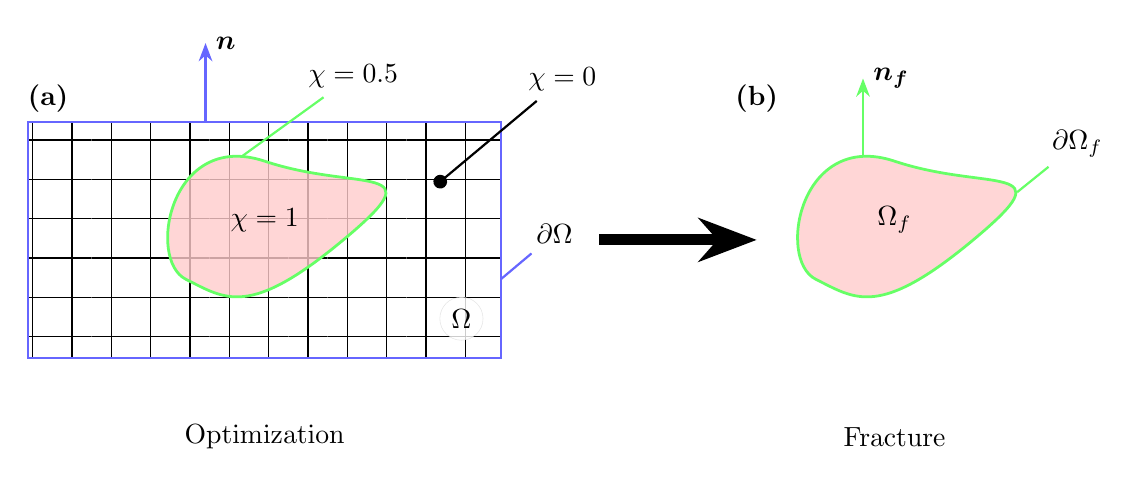
\begin{tikzpicture}
\begin{scope}
    \node[inner sep=0pt,minimum size=0pt] at (0.25cm,3.3cm) {\textbf{(a)}};
    \path[draw=blue!60!white,thick,pattern={Hatch[distance=0.5cm,line width=0.5pt,yshift=11.2pt,xshift=-2.5pt]},pattern color=black] (0,0) rectangle (6cm,3cm);
    \draw[line width=1pt,draw=green!60!white, fill=red!20!white, fill opacity=0.8] (2cm, 1cm) .. controls (2.5 cm, 0.75cm) and (2.8cm, 0.5cm) .. (4cm, 1.5cm) .. controls (5.2 cm, 2.5cm) and (4.2cm, 2.1cm) .. (3cm, 2.5cm) .. controls (1.8cm, 2.9cm) and (1.5cm, 1.25) .. (2cm,1cm);
    
    \node at (3cm, 1.75cm) [] {$\chi=1$};
    \node at (2.6cm, 2.48cm) [pin={[pin distance=1cm, pin edge={thick,draw=green!60!white}]45:{$\chi=0.5$}}] {};
    \node at (5.5cm, 0.5 cm) [circle,minimum size=4pt,inner sep=2pt, fill=white,draw=black, very thin,draw opacity=0.1, fill opacity=0.8,text opacity=1] {$\Omega$};
    \node at (6cm, 1cm) [inner sep=0pt,minimum size=0pt, pin={[pin edge={thick,draw=blue!60!white}]45:{$\partial\Omega$}}] {};
        \node at (5.04cm, 2.08cm) [pin={[pin distance=1.5cm, pin edge={Circle[]-,thick,draw=black}]45:{$\chi=0$}}] {};

    \draw[-Stealth,draw=blue!60!white,thick] (2.25cm,3cm) -- +(0,1cm) node[right] {$\boldsymbol{n}$};
    \node at (3cm, -1cm) [] {Optimization};
    \end{scope}

    \draw[-Stealth, line width=4pt] (7.25cm, 1.5cm) -- +(2cm,0);
    \begin{scope}[xshift=8cm]
            \node[inner sep=0pt,minimum size=0pt] at (1.25cm,3.3cm) {\textbf{(b)}};
            \draw[line width=1pt,draw=green!60!white, fill=red!20!white, fill opacity=0.8] (2cm, 1cm) .. controls (2.5 cm, 0.75cm) and (2.8cm, 0.5cm) .. (4cm, 1.5cm) .. controls (5.2 cm, 2.5cm) and (4.2cm, 2.1cm) .. (3cm, 2.5cm) .. controls (1.8cm, 2.9cm) and (1.5cm, 1.25) .. (2cm,1cm);

            \draw[-Stealth,draw=green!60!white,thick] (2.6cm,2.55cm) -- +(0,1cm) node[right] {$\boldsymbol{n_f}$};
    \node at (3cm, 1.75cm) [] {$\Omega_f$};
        \node at (4.55cm, 2.1cm) [inner sep=0pt,minimum size=0pt, pin={[pin edge={thick,draw=green!60!white}]45:{$\partial\Omega_f$}}] {};
        
\node at (3cm,-1cm ) []{Fracture};
    \end{scope}

    
\end{tikzpicture}
    \caption{Definition of the domains $\Omega$ and $\Omega_f$ used in the topology optimization and in fracture simulations respectively}
    \label{fig:omega_omega_f}
\end{figure}





The boundary value problem is described using the Hamilton
functional
\begin{equation}
	\label{eq:hamiltonian}
	\mathcal{H}[\boldsymbol{u},\chi,\phi]
	=\mathcal{G}[\boldsymbol{u},\chi,\phi]
	-\mathcal{D}[\chi,\phi]
	+\mathcal{C}[\chi,\phi]
	-\mathcal{R}[\chi,\phi]\;
\end{equation}
with $\boldsymbol{u}$ being the displacement field. The constituent
functionals are the Gibbs energy
\begin{equation}
	\label{eq:gibbs_ene}
	\mathcal{G}[\boldsymbol{u},\chi,\phi]
	=\int_{\Omega}\psi_e(\boldsymbol{u},\chi,\phi)\;\mathrm{d}V
	-\int_{\Omega}\boldsymbol{b}\cdot\boldsymbol{u}\;\mathrm{d}V
	-\int_{\partial\Omega}\boldsymbol{t}\cdot\boldsymbol{u}\;\mathrm{d}A\;,
\end{equation}
the dissipation functional, with dissipation functions $\Delta_\chi^\mathrm{diss}$ and $\Delta_\phi^\mathrm{diss}$ and the parameters for numerical damping $\eta_\chi$ and $\eta_\phi$, respectively
\cite{jantos_evolutionary_2016}
\begin{align}
	\label{eq:D}
	\mathcal{D}               & =
	\int_{\Omega}
	\frac{\partial\Delta_\chi^\mathrm{diss}}
	{\partial\dot{\chi}}\chi
	+\frac{\partial\Delta_\phi^\mathrm{diss}}
	{\partial\dot{\phi}}\phi\,\mathrm{d}V\;,
	\\
	\label{eq:delta_diss_chi}
	\Delta^\chi_\mathrm{diss} & =
	\frac{1}{2}\eta_{\chi}\dot{\chi}^2\;,
	\\
	\label{eq:delta_diss_phi}
	\Delta^\phi_\mathrm{diss} & =
	\frac{1}{2}\eta_{\phi}\dot{\phi}^2\;,
\end{align}
the regularization functional based on
\cite{jantos_accurate_2019}, with the regularization parameters
$\beta_{\chi}$ and $\beta_{\phi}$
\begin{equation}
	\label{eq:R}
	\mathcal{R}
	=\int_{\Omega}
	\frac{1}{2}\beta_{\chi}|\nabla\chi|^2
	+\frac{1}{2}\beta_{\phi}|\nabla\phi|^2
	\;\mathrm{d}V\;,
\end{equation}
and the constraint functional
\begin{equation}
	\mathcal{C}=\Lambda \left[
	\int_{\Omega}
	((1-\phi_\mathrm{min})\phi+\phi_\mathrm{min})
	\chi\;\mathrm{d}V-\rho\Omega\right]
	+\int_{\Omega}\gamma_{\chi}\chi+\gamma_{\phi}\phi
	\;\mathrm{d}V\;.
	\label{eq:C}
\end{equation}
The maximal structural volume constraint is
formulated using the Lagrange multiplier $\Lambda$, with
$0 < \rho < 1$ being a chosen value for the specific boundary value problem.
The interval bounds from
Eqs.~(\ref{eq:chi_def}) and~(\ref{eq:phi_def}) are applied using the
Karush-Kuhn-Tucker parameters $\gamma_\chi$ and $\gamma_\phi$.

The material behavior is described using the elastic strain
energy density
\begin{equation}
	\label{eq:psi}
	\psi_e=\frac{1}{2}\boldsymbol{\varepsilon}
	:\mathbb{C}(\chi,\phi):\boldsymbol{\varepsilon}\;,
\end{equation}
with the stiffness tensor
\begin{equation}
	\label{eq:E_eff}
	\mathbb{C}(\chi,\phi)
	=[(1-\kappa)\chi^p+\kappa]\,
	\mathbb{C}\!\left(E(\phi),\nu\right)
\end{equation}
with the small numerical parameter $\kappa = 10^{-9}$ to prevent
singularities. For the Young's modulus of the porous material,
we apply the mixture rule
\begin{equation}
	E(\phi)=(E_1-E_0)\phi^q+E_0 .
	\label{eq:E_phi}
\end{equation}
This material interpolation is based on the SIMP approach
\cite{bendsoe_optimal_1989}, with the exponents $p$ and $q$ and
Young's moduli $E_0$ and $E_1$ for fully porous and solid
material, respectively. The exponent $p$ serves as a
penalization factor to suppress intermediate gray densities
during the optimization and is usually chosen to be $p=3$.
In correspondence with the established Gibson-Ashby power law
\cite{gibson_mechanics_1982}, we set the exponent $q$ to
$q=2$. The Poisson ratio is kept constant as $\nu=0.3$ for all
cases in this work. The stiffness ratio of maximally porous
material to full material is generally chosen as
$E_0/E_1>\phi_\mathrm{min}$. In this work,
$\phi_\mathrm{min}=0.5$ and $E_0/E_1=0.6$.

The stiffness tensor $\mathbb{C}(E,\nu)$ is the isotropic
linear-elastic stiffness tensor defined by the Lam\'{e}
parameters $\lambda$ and $\mu$. Under the plane strain
assumption used for the fracture simulations, these parameters
are obtained from Young's modulus and Poisson ratio by
\begin{equation}
	\mu(\phi)=\frac{E(\phi)}{2(1+\nu)}, \qquad
	\lambda(\phi)=
	\frac{E(\phi)\nu}{(1+\nu)(1-2\nu)} .
	\label{eq:lame_from_E}
\end{equation}
Consequently, $\lambda$ and $\mu$ are local functions of the
porosity field through $E(\phi)$. For the solid material,
$E_1=210000~\mathrm{N}/\mathrm{mm}^2$ and $\nu=0.3$, which gives
$\mu_1=80769.23~\mathrm{N}/\mathrm{mm}^2$ and
$\lambda_1=121153.85~\mathrm{N}/\mathrm{mm}^2$. Since
$E_0/E_1=0.6$, the porous reference modulus is
$E_0=126000~\mathrm{N}/\mathrm{mm}^2$.

Finally, we apply the stationarity condition
\begin{equation}
	\label{eq:var_H}
	\delta\mathcal{H}=0
\end{equation}
and obtain the resulting evolution equations in their strong
form with their respective homogeneous Neumann boundary conditions:
\begin{align}
	\label{eq:evol_chi}
	 \dot{\chi} &
	=\frac{1}{\eta_{\chi}}
	(p_\chi-\Lambda((1-\phi_\mathrm{min})\phi+\phi_\mathrm{min})
	-\gamma_\chi+\beta_\chi\nabla^2\chi)\;,
	\\
	0          & = \beta_\chi\,\nabla\chi\cdot\boldsymbol{n}\;,   \\
	\label{eq:evol_phi}
	 \dot{\phi} &
	=\frac{1}{\eta_{\phi}}
	(p_\phi-\Lambda(1-\phi_\mathrm{min})\chi-\gamma_\phi
	+\beta_{\phi}\nabla^2\phi)\;,
	\\
	0          & = \beta_{\phi}\,\nabla\phi\cdot\boldsymbol{n}\;,
\end{align}
Here and in the following, the dot denotes the material time
derivative, e.g., $\dot{\chi}=\mathrm{d}\chi/\mathrm{d}t$,
where $t$ is the time. Furthermore,
$p_\chi$ and $p_\phi$ are the driving forces
(sensitivities), i.e.,
\begin{align}
	p_\chi & =-\frac{\partial\psi_e(\chi,\phi)}
	{\partial\chi}\;, \\
	p_\phi & =-\frac{\partial\psi_e(\chi,\phi)}
	{\partial\phi}\;,
\end{align}
where $\boldsymbol{n}$ denotes the outward pointing normal vector
on the design space.
The optimization problem therefore consists of the balance of
linear momentum, derived from the Gibbs energy and from the
evolution equations (\ref{eq:evol_chi}) and (\ref{eq:evol_phi}).
These are solved in a staggered manner, as has been described in
detail in \cite{jantos_accurate_2019}. The discretized balance
of linear momentum is solved using standard finite element
analysis with first-order Lagrange finite elements on a
structured quadrilateral mesh. Both $\chi$ and $\phi$ are defined
as element-wise constant. The topology optimization has been
implemented in the programming language Julia \citep{Julia-2017}
with the use of the finite elements package Ferrite.jl
\citep{Carlsson_Ferrite_jl}.

\subsection{A phase field model of brittle
	fracture}\label{sec:phase_field}
The phase field model for quasi-static brittle fracture
described in \cite{kuhn_continuum_2010} is employed to compute
the crack evolution in the optimized structures.
This means that dynamic effects that might be relevant to
capture the real microscopic fracture behavior even under
quasi-static macroscopic loading conditions are neglected.
In this section, the employed phase field model is briefly
introduced.
% and two key characteristics of the model: consistence with the
% Griffith-criterion and the ability to model stress driven crack
% nucleation in undamaged material are highlighted.

We consider a linear elastic body $\Omega_f$  with local
Lam\'{e} parameters $\lambda(\phi)$ and $\mu(\phi)$ and local
energetic (Griffith) fracture resistance $G_c(\phi)$. The Lam\'{e} parameters follow from
Young's modulus field $E(\phi)$ and constant Poisson ratio
$\nu=0.3$ introduced in Eqs.~(\ref{eq:E_phi})
and~(\ref{eq:lame_from_E}). The displacement is denoted as
$\boldsymbol{u}$ and Dirichlet $\boldsymbol{u}^*$ and/or
Neumann boundary conditions $\boldsymbol{t}^*$ may be prescribed
at the boundary
$\partial\Omega_f=\partial\Omega_f^u\bigcup\partial\Omega_f^t$.
Cracks within $\Omega_f$ are represented in a regularized manner by a phase
field $s\in\left[0,1\right]$.
The phase field assumes the value $s=0$ at cracks and grows
continuously to $s=1$ away from the crack. The width of the
transition zone is controlled by the parameter~$\beta_s$. {This
		internal length scale needs to be small compared to the
		geometrical features of the body in order to properly resolve
		them -- and their effect on crack propagation -- in
		the fracture
		simulation.}
By means of this additional field, the sum of the elastic energy
based on the density $\psi_e$ and the fracture energy is
approximated by the functional
\begin{equation}
	\Pi\left[\nabla{\boldsymbol{u}},\boldsymbol{u},
	\nabla{s},s\right] =
	\Pi_\mathrm{el} + \Pi_\mathrm{frac} -
	\int_{\partial\Omega_f^t}\boldsymbol{t}^*\cdot{\boldsymbol{u}}
	\,{\rm{d}}A,
\end{equation}
where
\begin{equation}
	\Pi_\mathrm{frac} =
	\int_{\Omega_f} G_c(\phi(\boldsymbol{x})) \left( \dfrac{
			\left(1-s\right)^2}{4\beta_s} +
	\beta_s\left|\nabla{s}\right|^2 \right) \,{\rm{d}}V
\end{equation}
is the fracture energy associated with the creation of
regularized crack surfaces. The local fracture resistance
$G_c(\phi(\boldsymbol{x}))$ enters the integrand because it varies with
the local porosity field in this work,
\begin{equation}
	\Pi_\mathrm{el}=\int_{\Omega_f} \left[
		\left(s^2+\kappa_s\right)\psi_e^+ + \psi_e^- \right] \,{\rm{d}}V
	\label{eq:elastic_energy}
\end{equation}
is the elastic energy and $\kappa_s$ controls the residual stiffness
in broken material.
The elastic energy density is split into tensile and compressive
contributions following the spectral decomposition proposed by
Miehe et al.~\cite{miehe_phase_2010}. With
\begin{align}
	\boldsymbol{\varepsilon}                       & =
	\text{sym}\left(\nabla{\boldsymbol{u}}\right), &
	\boldsymbol{\varepsilon}                       & =
	\sum_{i=1}^{n}\varepsilon_i\,
	\boldsymbol{N}_i\otimes\boldsymbol{N}_i,
	                                               &
	 \boldsymbol{\varepsilon}^{\pm}                 & =
	\sum_{i=1}^{n}\left<\varepsilon_i\right>_{\pm}
	\boldsymbol{N}_i\otimes\boldsymbol{N}_i,
\end{align}
where $\varepsilon_i$ and $\boldsymbol{N}_i$ are the eigenvalues
and eigenvectors of $\boldsymbol{\varepsilon}$, respectively.
The two energy densities are written as
\begin{equation}
	\psi_e^{\pm} =
	\dfrac{1}{2}\lambda
	\left<\text{tr}\left(\boldsymbol{\varepsilon}\right)
	\right>_{\pm}^2
	+
	\mu\,\text{tr}
	\left(\left(\boldsymbol{\varepsilon}^{\pm}\right)^2\right).
\end{equation}
Here, $\left<*\right>_+ = \text{max}(0,*)$ and $\left<*\right>_-
	= \text{min}(0,*)$. Only the tensile part $\psi_e^+$ is degraded
by the phase field, see Eq.~(\ref{eq:elastic_energy}), which suppresses crack growth in compression
while still allowing crack closure. The residual stiffness is
chosen as $\kappa_s=0.001$ for all simulations in this work.
The field equations for the displacement $\boldsymbol{u}$ and
the phase field $s$ are found from the variational principle
\begin{equation}
	\delta{\Pi} = 0,
\end{equation}
which corresponds to the following Euler-Lagrange equations
\begin{align}
	\begin{split}
		&\text{div}\boldsymbol{\sigma}=\boldsymbol{0}
		\quad\text{with}\quad \boldsymbol{\sigma} =
		\left(s^2+\kappa_s\right)\left[
			\lambda\left<\text{tr}
			\left(\boldsymbol{\varepsilon}\right)\right>_+
			\boldsymbol{1}
			+ 2\mu\boldsymbol{\varepsilon}^+\right] +
		\lambda\left<\text{tr}
		\left(\boldsymbol{\varepsilon}\right)\right>_-
		\boldsymbol{1}
		+ 2\mu\boldsymbol{\varepsilon}^-\quad \text{in} \, \Omega_f, \\
		&{\boldsymbol{\sigma} \boldsymbol{n}_f =\boldsymbol{t}^*}
		\quad\text{on}\,\partial\Omega_f^t,\\
		-&\dfrac{\dot{s}}{M} =
		2s\psi_e^+-G_c
		\left[2\beta_s\Delta{s}
			+\dfrac{1-s}{2\beta_s}\right]
		\quad \text{in} \, \Omega_f, \\
		&\nabla{s}\cdot{\boldsymbol{n}_f} =
		0\quad\text{on}\,\partial\Omega_f,
	\end{split}
	\label{eq:field_equations}
\end{align}
with the outward normal vector of the fracture domain $\boldsymbol{n}_f$.
The regularization (in time) term $-\nicefrac{\dot{s}}{M}$ is
added to enable a stable numerical
solution in case of  crack nucleation in undamaged material. The
mobility parameter $M$ controls the rate at which cracks can
grow in the given model. The
mobility is chosen as
$M=\text{100}~\mathrm{mm}^3/(\mathrm{Nmm}\,\mathrm{s})$.

Besides energy-driven crack growth from existing cracks, the
phase-field model also permits stress-driven crack nucleation in
undamaged material. For the one-dimensional case, the
corresponding critical stress follows from the analytical
investigation by Kuhn~\cite{kuhn_numerical_2013} as
\begin{equation}
	\sigma_c = \frac{9}{16}\sqrt{\frac{\mu G_c}{3\beta_s}}.
	\label{eq:sigma_c_1d}
\end{equation}
This relation couples the shear modulus $\mu$, the fracture
resistance $G_c$, and the regularization length $\beta_s$. In
the present work, it is used as a local estimate of
the nucleation strength by evaluating Eq.~(\ref{eq:sigma_c_1d})
with the local material fields.

In addition, we model the irreversibility of crack growth by
setting Dirichlet boundary conditions
\begin{equation}
	s\left(\boldsymbol{x},t>t_{\boldsymbol{x}}\right) =
	0\quad\text{if}\quad{s}
	\left(\boldsymbol{x},t_{\boldsymbol{x}}\right)=0
\end{equation}
once the phase field has assumed $s=0$ for the first time
$t_{\boldsymbol{x}}$ at a given point $\boldsymbol{x}$.

In order to solve the coupled field
equations~(\ref{eq:field_equations}) we employ first-order
Lagrange finite elements on triangular meshes. The displacement
field and the phase field are solved as a monolithic nonlinear
system with a Newton method. The phase-field evolution is
discretized in pseudo-time by an implicit Backward-Euler scheme,
so that the time derivative at step $n$ is approximated by
\begin{equation}
	\dot{s}_n \approx \frac{s_n-s_{n-1}}{\Delta t}.
\end{equation}
An adaptive time-stepping procedure is used, starting with a
maximum time increment of $\Delta t=0.001~\mathrm{s}$: if the
Newton iteration does not converge for a time increment, the
previous converged state is restored, $\Delta t$ is reduced by a
factor of two, and the increment is repeated. All simulations
are continued until Newton convergence can no longer be obtained
under further time-step reduction, i.e., when
$\Delta t<10^{-14}~\mathrm{s}$.

\subsubsection{Fracture toughness as a function of porosity}

The dependence of the stiffness on porosity is described by
Eq.~(\ref{eq:E_eff}). In the following failure simulations,
based on the phase-field model introduced in
Section~\ref{sec:phase_field}, we additionally account for a
dependence of the fracture resistance \( G_c \) on the local
porosity $\phi_r$. This relation is applied only after topology
optimization to assess the fixed designs; \(G_c\) does not enter
the optimization problem.

The relationship between fracture resistance and local
porosity is given by
\begin{equation}
	\frac{G_c(\phi_r)}{G_{c}^0}
	= \min\left( \max\left(
		A - B \exp\left(-C \left[\sqrt{\frac{\pi}{4(\phi_r)}} -
				1\right]\right),
		0.1 \right),
	1.0 \right)\;.
	\label{eq:gc_porosity_relation}
\end{equation}
The local porosity of the material is obtained from the
optimized porosity design field as
\begin{equation}
	\phi_r
	= \frac{\text{volume of voids}}{\text{total volume}}
	= - (1-\phi_{\text{min}})\phi
	+ (1-\phi_{\text{min}}).
	\label{eq:local_material_porosity}
\end{equation}
Here, the reference fracture toughness is
$G_c^0=1~\mathrm{Nmm}/\mathrm{mm}^2$, and
$(1-\phi_{\text{min}})=0.5$ is the maximum porosity allowed in
the material.
The parameters are \( A = 1.26 \), \( B = 0.78 \), and \(
C = 1.35 \).

This relation, depicted in Fig.~\ref{fig:gc_porosity_relation}, including the chosen parameter values
is motivated by the findings
in~\cite{schluter_determination_2025a} from numerical studies on
the effective fracture toughness of a simplified porous medium
with circular pores.

\begin{figure}[htbp]
	\centering

	\includegraphics[
		width=0.55\textwidth
	]{Images_A02/circular_fit_porosity_isolated.png}
	\caption{Normalized fracture toughness $G_c/G_c^{0}$ as a
	function of porosity $\phi_r$ based on the fitted circular-pore
	relation.}
	\label{fig:gc_porosity_relation}
\end{figure}

It provides a phenomenological description of the fracture
resistance as a function of the local porosity \( \phi_r \),
which is derived from the optimized porosity field \( \phi \)
only for the subsequent fracture assessment.
% The
% exponential term captures the saturation behavior associated
% with increasing wall thickness (i.e., increasing relative
% density), while the clipping ensures physically admissible
% bounds, limiting the fracture toughness to a minimum of 10\% and
% a maximum of 100\% of the fully dense material.

\section{Results}\label{sec_results}
This section first presents the topology-optimized structures
and evaluates their fracture response for the reference
porosity-gradient scale $\beta_{\phi}=0.01~\mathrm{mm^2}$. Its influence is then assessed by comparing the
\Evar structures for
$\beta_{\phi}\in\{0.001,0.01,0.05\}~\mathrm{mm^2}$.
\begin{figure}[htbp]
	\centering

	\resizebox{0.5\textwidth}{!}{%
		\input{Images_A02/cdb_setup.pdf_t}
		% your LaTeX figure file
	}
	\caption{Boundary value problem for topology optimization.}
	\label{fig:dcb_setup}
\end{figure}

% Prescribed displacement $u^*=(0,-1)$ is applied in the top
% right corner on a section $0.2~\mathrm{mm}$ long (see Fig.
% \ref{fig:bvp_sketch}). ?? needs to be described by A03 ??
% \begin{figure}[htp]
%     \centering
%     \begin{tikzpicture}
%     \coordinate (A) at (0,0);
%     \coordinate (U) at (0,2);
%     \coordinate (L) at (5,0);
%     \coordinate (B) at (5,2);

%     \draw[black,thick] (A) rectangle (B);
%     \begin{scope}[transform canvas={xshift=-2}]
%         \draw[thick] (A) +(0,-0.1) -- (U) -- ++(0,0.1);
%     \foreach \y in {-0.1,0.1,...,2.2}
%     {
%         \draw[] (0,\y)-- ++(-135:0.2);
%     }

%     \end{scope}
%     \draw[thick] (L) ++(0,-0.1) -- ++(-0.6,0);
% % \path[pattern={Lines[angle=45,distance=4,xshift=2.2]}] (L)
% ++(0,-0.1) -- ++(-0.5,0) -- ++(0,-0.2) -- ++ (0.5,0) --cycle;
%     \foreach \x in {5.0,4.85,...,4.3}
%     {
%         \draw[] (\x,-0.1) -- ++(-135:0.2);
%     }

%     \draw[] (U) ++(0,0.1) -- ++(0.6,0);
%     \foreach \x in {0,0.2,...,0.6}
%     {
%             \draw[{Triangle}-] (\x,2.1) -- (\x,2.6);
%     }
% \draw[|{Triangle}-{Triangle}|] (5.5,0) -- ++(0,2) node[midway,
% left] {b};
% \draw[|{Triangle}-{Triangle}|] (0,-1.4) -- ++(5,0) node[midway,
% above] {a};
% \draw[|{Triangle}-{Triangle}|] (4.4,-0.8) -- ++(0.6,0)
% node[midway, above] {0.2};
% \draw[|{Triangle}-{Triangle}|] (0,3.0) -- ++(0.6,0)
% node[midway, above] {0.2};

%     \node at (1.7,2.6) {$u^*=(0,-1)$};
% \node at (4.7,0) [pin={[pin distance=1cm,pin
% edge={black,shorten <= 0pt}]-10:$u_y=0$}] {};
% \node at (0.0,1) [pin={[pin edge={black,shorten <=
% -3pt}]-135:$u_x=0$}] {};
%     \node at (2.5,1) {Design space $\Omega$};
% \end{tikzpicture}

%     \caption{Boundary value problem}
%     \label{fig:bvp_sketch}
% \end{figure}

\subsection{Generation of topology optimized structures}
\label{sec:optimized_structures}

The boundary value problem investigated in this work, shown in
Fig.~\ref{fig:dcb_setup}, is a rectangular domain of
length $a=6~\mathrm{mm}$ and height $b=1~\mathrm{mm}$ that is fixed at the left and right
edges.
Prescribed discrete loads of $\boldsymbol{F}=-1~\mathrm{N}\boldsymbol{e}_y$ are
applied at the top edge at locations ($x=2~\mathrm{mm}$, $y=1~\mathrm{mm}$) and
($x=4~\mathrm{mm}$, $y=1~\mathrm{mm}$).

The damping parameters $\eta_\chi$ and $\eta_\phi$ are chosen from preliminary parameter studies. The parameter $\beta_\chi$ influences the minimal structural member size ($\sqrt{\beta_\chi}$ corresponds to the member thickness, as described in \cite{jantos_accurate_2019}) and $\beta_\phi$ is a scale parameter describing the width of the porous transition zone, i.e., the gradient steepness. As these parameters are problem dependent, an adaptive numerical procedure is used, which is described in detail in \cite{pravda_macroscopic_2026}.

The maximal structural volume has been chosen to be either $\rho=0.3$ or $\rho=0.6$, which leads to two sets of distinctive topologies and porosity distributions. All of the parameter values are gathered in Table \ref{tab:topopt_param}, with $n$ and $m$ being the number of finite elements in $x$ and $y$ direction respectively.

\begin{table*}[!htbp]
    \centering

    \begin{tabular}{cccccc}
        $n$ & $m$ & $\beta_\chi~[\mathrm{mm^2}]$
        & $\beta_\phi~[\mathrm{mm^2}]$ & $\eta_\chi~[\mathrm{s}]$
        & $\eta_\phi~[\mathrm{s}]$ \\
        \hline
        600 & 100 & 0.0009 & 0.01 & 14.0 & 150.0 \\
        \addlinespace
        $\phi_0$ & $p$ & $q$ & $\tfrac{E_0}{E_1}$ & $\rho$
        & $\phi_\mathrm{min}$ \\
        \hline
        0.5 & 3.0 & 2.0 & 0.6 & $\{0.3, 0.6\}$ & 0.5
    \end{tabular}
    \caption{{Parameter values used for the topology optimization}}

     \label{tab:topopt_param}
\end{table*}

The design domain is discretized using first-order Lagrange finite elements on quadrilateral meshes, with the design variables element-wise constant.
To solve the optimization problem, we make use of a staggered approach shown in Fig. \ref{fig:to_schema}. For the solution of the evolution equations, the strains are considered to be constant. A detailed description of the algorithm can be found in \cite{jantos_accurate_2019}. The convergence criteria are a relative change in the goal function
\begin{equation}
    \frac{\Psi_e^{i}-\Psi_e^{i-1}}{\Psi_e^{i}}\leq\Psi_\mathrm{tol}=10^{-4}\;,
\end{equation}
as well as the maximum norm of the change of both design variables
\begin{align}
    L_\infty(\Delta\chi)&\leq L_\infty^\mathrm{tol}=10^{-3}\\
    L_\infty(\Delta\phi)&\leq L_\infty^\mathrm{tol}=10^{-3}\; .
\end{align}
Further details regarding the numerical procedure and the choice of parameters can be found in \cite{pravda_macroscopic_2026}.
\begin{figure}
    \centering
    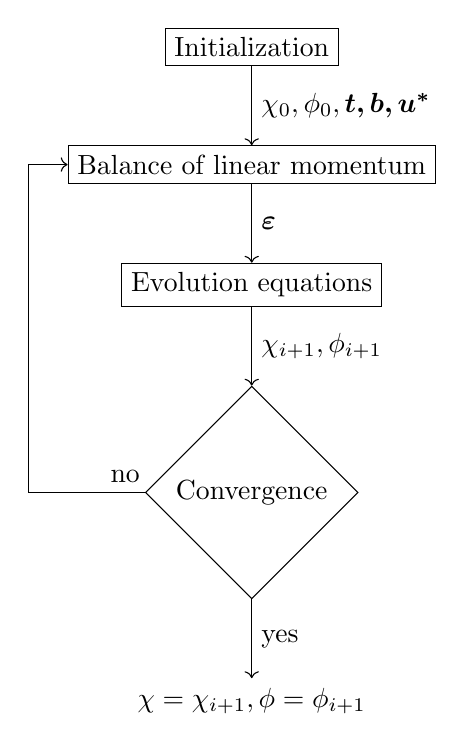
\begin{tikzpicture}

  \node (init)   [rectangle,draw=black]                     {Initialization};
  \node (FEM)   [rectangle,draw=black,below=of init]           {Balance of linear momentum};
  \node (TO) [rectangle,draw=black,below=of FEM]           {Evolution equations};
  \node (conv) [diamond,draw=black,below=of TO]         {Convergence};
  \node (end) [below=of conv] {$\chi=\chi_{i+1},\phi=\phi_{i+1}$};

  \path[->] (init) edge node [right] {$\chi_0,\phi_0,\boldsymbol{t,b,u^*}$} (FEM)
            (FEM) edge node [right] {$\boldsymbol{\varepsilon}$} (TO)
            (TO) edge node [right] {$\chi_{i+1},\phi_{i+1}$} (conv)
            (conv) edge node [right] {yes} (end);
  \draw[->] (conv.west) -- node [midway,above] {no} ++ (-0.5,0) -|  ($(FEM.west) - (0.5,0)$)    -- (FEM.west);

    \end{tikzpicture}
    \caption{Schematic of the optimization algorithm}
    \label{fig:to_schema}
\end{figure}

In total three sets of optimized structures for the boundary
value problem depicted in Fig.~\ref{fig:dcb_setup}
were computed.
The three sets are denoted by \Evar, \Emin, and \Emax. The set
\Evar allows for a locally varying porosity distribution
$\phi$ as described in Section~\ref{sec:topology_optimization}.
The set \Emin has the homogeneous porosity distribution
$\phi=0$, corresponding to maximal physical porosity, while
\Emax has the homogeneous distribution $\phi=1$, corresponding
to no physical porosity.
We guarantee by constraint~(\ref{eq:C}) that the
same overall mass is applied for all three sets. 
% This means that the (dimensionless) mass
% \begin{equation}
% 	m=\rho\Omega=\int_{\Omega}
% 	((1-\phi_\mathrm{min})\phi+\phi_\mathrm{min})
% 	\chi\;\mathrm{d}V
% 	\label{eq:mass_constraint}
% \end{equation}
% is constant across sets. 
Therefore, the two sets with homogeneous porosity distribution are equivalent to structures optimized only with the density distribution as a design variable, with different Young's Modulus for the full material, and serve as a comparison to the third set where both density and porosity distribution have been solved for.
The resulting \Evar fields are shown in
Figs.~\ref{fig:to_E_var_rho_03}
and~\ref{fig:to_E_var_rho_06}, while the homogeneous-porosity
reference fields are summarized in
Fig.~\ref{fig:to_E_min_max_rho_03_06}.

The density and porosity distributions of the resulting
structures for \Evar
are depicted in Figs.~\ref{fig:to_E_var_rho_03}
and~\ref{fig:to_E_var_rho_06}. The resulting topology conforms
to the loading conditions, forming a truss-like structure, with members in the directions of the
force paths. The effective Young's modulus field shown in the
bottom rows is computed from the local porosity distribution~$\phi$ using Eq.~(\ref{eq:E_phi}). For \Emin and \Emax,
shown in Fig.~\ref{fig:to_E_min_max_rho_03_06}, the modulus is
homogeneous with $E=E_0$ and $E=E_1$, respectively, whereas for
\Evar it varies spatially according to the optimized porosity
field. In all cases, truss-like structures emerge, which is
expected for the double cantilever beam problem.

As visible in Figs.~\ref{fig:to_E_var_rho_03}
and~\ref{fig:to_E_var_rho_06}, areas with high strains and
thus high elastic strain energy are filled with full material,
whereas the rest of the structure consists of maximally porous
material. More material is employed in the regions around the
points of force application and at the top and bottom of the
fixed boundaries. Discrete forces naturally lead to stress
concentrations, which are mitigated by the optimization by
placing more material in those regions. In addition, the domain
is mostly subject to bending, with the moment and the
associated stress expected to be highest at the top and bottom
of the fixed boundaries, which is also reflected in the
stiffness distribution.

One reason for the porosity distribution is the choice of
$\frac{E_0}{E_1}$: maximally porous material has a favorable
ratio of stiffness to volume and is thus preferred where
possible, as reflected by the broad low-stiffness regions in
the bottom rows of Figs.~\ref{fig:to_E_var_rho_03}
and~\ref{fig:to_E_var_rho_06}. The second reason is related to
the loading conditions, where bending plays a dominant role.
Employing porous material is beneficial, as it uses up less of
the available volume and allows for wider structural members.
This in turn leads to a higher second moment of area, which
scales with the fourth power, compared to the stiffness, which
scales only quadratically.

Optimization for set \Evar yields minimum (no) physical porosity
($\phi=1$) and thus maximum stiffness only at very localized
regions around the points of force application and at the
corners of the domain. In most of the domain, the maximum
physical porosity ($\phi=0$), i.e. minimum stiffness, is
obtained, as shown in the porosity and modulus rows of
Figs.~\ref{fig:to_E_var_rho_03}
and~\ref{fig:to_E_var_rho_06}.

\begin{figure}
    \centering
    \begin{overpic}[width=\linewidth]{Images_A03/beta_0_01_a_6_rho_0_3_chi_phi_E_no_legend.png}
        \put(101.2,36){\rotatebox{90}{\makebox[5em][c]{\large$\chi$}}}
        \put(101.2,20){\rotatebox{90}{\makebox[5em][c]{\large$\phi$}}}
        \put(101.2,-1){\rotatebox{90}{\makebox[8.5em][c]{\small$E\ [\mathrm{N/mm}^2]$}}}
    \end{overpic}
    \caption{Results for the set \Evar with $\rho=0.3$. Top to
    bottom: relative density $\chi$, porosity $\phi$, and
    effective Young's modulus $E$.}
    \label{fig:to_E_var_rho_03}
\end{figure}

\begin{figure}
    \centering
    \begin{overpic}[width=\linewidth]{Images_A03/beta_0_01_a_6_rho_0_6_chi_phi_E_no_legend.png}
        \put(101.2,36){\rotatebox{90}{\makebox[5em][c]{\large$\chi$}}}
        \put(101.2,20){\rotatebox{90}{\makebox[5em][c]{\large$\phi$}}}
        \put(101.2,-1){\rotatebox{90}{\makebox[8.5em][c]{\small$E\ [\mathrm{N/mm}^2]$}}}
    \end{overpic}
    \caption{Results for the set \Evar with $\rho=0.6$. Top to
    bottom: relative density $\chi$, porosity $\phi$, and
    effective Young's modulus $E$.}
    \label{fig:to_E_var_rho_06}
\end{figure}

\begin{figure}
    \centering
    \begin{overpic}[width=\linewidth]{Images_A03/beta_0_01_a_6_rho_0_3_0_6_min_max_E_no_legend.png}
        \put(101.2,31){\rotatebox{90}{\makebox[8.5em][c]{\small$E\ [\mathrm{N/mm}^2]$}}}
        \put(101.2,15){\rotatebox{90}{\makebox[8.5em][c]{\small$E\ [\mathrm{N/mm}^2]$}}}
        \put(101.2,-1){\rotatebox{90}{\makebox[8.5em][c]{\small$E\ [\mathrm{N/mm}^2]$}}}
    \end{overpic}
    \caption{Results for the sets \Emin (top, for $\rho=0.3$)
    and \Emax (middle, for $\rho=0.3$ and bottom, for
    $\rho=0.6$). Only the effective Young's modulus $E$ is shown.}
    \label{fig:to_E_min_max_rho_03_06}
\end{figure}

% \begin{figure}[htb]
%     \centering
% \begin{overpic}[width=1.0\textwidth]{Images_A02/density_var_5_1
% 0_15_20.png}
%         \put(5,22){\textbf{(a)}}
%         \put(55,22){\textbf{(b)}}
%         \put(5,05){\textbf{(c)}}
%         \put(55,05){\textbf{(d)}}
%     \end{overpic}
% \caption{Density plot $\chi$ for \Evar for $a = 5, 10, 15, 20$}
%     \label{fig:density_var}
% \end{figure}

% \begin{figure}[htb]
%     \centering
% \begin{overpic}[width=1.0\textwidth]{Images_A02/porosity_raw_va
% r_5_10_15_20.png}
%         \put(5,22){\textbf{(a)}}
%         \put(55,22){\textbf{(b)}}
%         \put(5,05){\textbf{(c)}}
%         \put(55,05){\textbf{(d)}}
%     \end{overpic}
% \caption{Porosity distribution $\phi$ for \Evar for $a = 5, 10,
% 15, 20$}
%     \label{fig:porosity_distribution_var}
% \end{figure}

% \begin{figure}[htb]
%     \centering
% \begin{overpic}[width=1.0\textwidth]{Images_A02/density_min_5_1
% 0_15_20.png}
%         \put(5,22){\textbf{(a)}}
%         \put(55,22){\textbf{(b)}}
%         \put(5,05){\textbf{(c)}}
%         \put(55,05){\textbf{(d)}}
%     \end{overpic}
% \caption{Density plot $\chi$ for \Emin for $a = 5, 10, 15, 20$}
%     \label{fig:density_min}
% \end{figure}

% \begin{figure}[htb]
%     \centering
% \begin{overpic}[width=1.0\textwidth]{Images_A02/porosity_raw_mi
% n_5_10_15_20.png}
%         \put(5,22){\textbf{(a)}}
%         \put(55,22){\textbf{(b)}}
%         \put(5,05){\textbf{(c)}}
%         \put(55,05){\textbf{(d)}}
%     \end{overpic}
% \caption{Porosity distribution $\phi$ for \Emin for $a = 5, 10,
% 15, 20$}
%     \label{fig:porosity_distribution_min}
% \end{figure}

For the set \Emax, the optimization yields distinctively
different truss structures as can be observed in the contour
plots in Fig.~\ref{fig:to_E_min_max_rho_03_06}. In general,
fewer and thinner members of the truss are generated. The
physical porosity is however zero everywhere, i.e., solid
material $\phi=1$. Since more material is employed for
$\rho=0.6$ than for $\rho=0.3$, the corresponding structures
are more massive. For \Emin and $\rho=0.6$, the constraint
(\ref{eq:C}) cannot be fulfilled, so that no optimized
structure is obtained for this combination. Table
\ref{tab:TO_Psi_comp} displays the final structural compliance
values for the three investigated sets for $\rho=\{0.3,0.6\}$.
The stiffness gain for $\rho=0.3$ is around $2.5\%$ and around
$8\%$ for $\rho=0.6$, proving that optimizing the porosity
distribution leads to increased structural performance.

\begin{table}[]
    \centering
    \begin{tabular}{ccc}
         & $\rho=0.3$&$\rho=0.6$  \\
         \hline
         \Emin & $4.0665\cdot10^{-7}$& - \\
         \hline
         \Emax & $4.7695\cdot10^{-7}$ & $2.4374\cdot10^{-7}$ \\
         \hline
         \Evar & $3.9618\cdot10^{-7}$ & $2.2436\cdot10^{-7}$
    \end{tabular}
    \caption{Comparison of final structural compliance values for the three investigated sets for $\rho={0.3,0.6}$ and $\beta_{\phi}=0.01~\mathrm{mm^2}$}
    \label{tab:TO_Psi_comp}
\end{table}

% \begin{figure}[htb]
%     \centering
% \begin{overpic}[width=1.0\textwidth]{Images_A02/density_max_5_1
% 0_15_20.png}
%         \put(5,22){\textbf{(a)}}
%         \put(55,22){\textbf{(b)}}
%         \put(5,05){\textbf{(c)}}
%         \put(55,05){\textbf{(d)}}
%     \end{overpic}
% \caption{Density plot $\chi$ for \Emax for $a = 5, 10, 15, 20$}
%     \label{fig:density_max}
% \end{figure}

% \begin{figure}[htb]
%     \centering
% \begin{overpic}[width=1.0\textwidth]{Images_A02/porosity_raw_ma
% x_5_10_15_20.png}
%         \put(5,22){\textbf{(a)}}
%         \put(55,22){\textbf{(b)}}
%         \put(5,05){\textbf{(c)}}
%         \put(55,05){\textbf{(d)}}
%     \end{overpic}
% \caption{Porosity distribution $\phi$ for \Emax for $a = 5, 10,
% 15, 20$}
%     \label{fig:porosity_distribution_max}
% \end{figure}

\subsection{Failure behavior of topology optimized structures}

In this section, we investigate the optimized structures from
Section~\ref{sec:topology_optimization} with regard to their resistance to failure
due to brittle fracture. In order to model such failure, we
employ the phase field model from Section~\ref{sec:phase_field}.

For the fracture simulations, we restrict the analysis to the
subdomain in which the relative density $\chi$ exceeds 0.5
\begin{equation}
	\Omega_f = \{\, x \in \Omega \mid \chi(x) \geq 0.5 \,\},
	\label{eq:omega_f}
\end{equation}
where $\Omega_f \subset \Omega$ and re-mesh that domain with
first-order Lagrange finite elements on triangular meshes, see also Fig.~\ref{fig:omega_omega_f}.

\begin{figure}[htbp]
	\centering

	\includegraphics[
		width=0.80\textwidth
	]{Images_A02/rho_omega_constraint.png}
	\caption{Evaluation of the volume-constraint integral in
		Eq.~(\ref{eq:C}) on the five generated
		fracture domains $\Omega_f$. The relative density field is
		set to $\chi=1$ on $\Omega_f$, and the porosity design
		variable $\phi$ is reconstructed from the Young's modulus
		field using Eq.~(\ref{eq:E_phi}).}
	\label{fig:rho_omega_constraint}
\end{figure}

Fig.~\ref{fig:rho_omega_constraint} confirms that extracting
and re-meshing the fracture domain $\Omega_f$ according to
Eq.~(\ref{eq:omega_f}) preserves the mass constraint from
Eq.~(\ref{eq:C}) for the investigated
structures: the integral
$\int_{\Omega_f}((1-\phi_\mathrm{min})\phi
+\phi_\mathrm{min})\,\mathrm{d}V$ recovers the prescribed
value $\rho\Omega$. Small deviations are attributed to the
discretized geometry and the interpolation of the material
field.
\resultfigurediscussion

In the fracture simulations, very similar boundary conditions to
the topology optimization boundary value problem are employed.
The left and right edges of the domain are fixed in both
directions, i.e.,
\[
	u_x = 0, \quad u_y = 0,
\]
with the coordinate system oriented as shown in
Fig.~\ref{fig:dcb_setup}. The load at the top boundary is
applied by prescribing displacement boundary conditions
\[
	u_y^*(t) = -t v_0, \quad v_0 = 1~\mathrm{mm}/\mathrm{s},
\]
with $t$ being the time measured in seconds and $v_0$
the prescribed displacement rate. The displacement is applied on
two strips of width $w = 0.075~\mathrm{mm}$ at the top of the
domain, defined mathematically as
\begin{equation}
	\partial\Omega_{\mathrm{L}} =
	\left\{ (x,y) \,\Big|\, 1.9625~\mathrm{mm} \le x \le
	2.0375~\mathrm{mm},\; y=1~\mathrm{mm} \right\},
	\label{eq:left_strip}
\end{equation}
\begin{equation}
	\partial\Omega_{\mathrm{R}} =
	\left\{ (x,y) \,\Big|\, 3.9625~\mathrm{mm} \le x \le
	4.0375~\mathrm{mm},\; y=1~\mathrm{mm} \right\},
	\label{eq:right_strip}
\end{equation}

The total-boundary external work reported below is evaluated
from the boundary tractions of the fracture solution over the
complete boundary of the fracture domain. With
$\boldsymbol{t}=\boldsymbol{\sigma}\boldsymbol{n}_f$, it is
defined as the accumulated traction power
\begin{equation}
	W(t) =
	\int_{0}^{t}
	\int_{\partial\Omega_f}
	\left(\boldsymbol{\sigma}(\boldsymbol{x},\tau)
	\boldsymbol{n}_f\right)
	\cdot\dot{\boldsymbol{u}}(\boldsymbol{x},\tau)
	\,\mathrm{d}A\,\mathrm{d}\tau .
	\label{eq:total_boundary_work}
\end{equation}
Numerically, the work increment between two stored states is
computed directly from the stress expression by trapezoidal
integration,
\begin{equation}
	\Delta W_n =
	\frac{1}{2}
	\int_{\partial\Omega_f}
	\left[
	\boldsymbol{\sigma}_n\boldsymbol{n}_f
	+\boldsymbol{\sigma}_{n-1}\boldsymbol{n}_f
	\right]\cdot
	\left(\boldsymbol{u}_n-\boldsymbol{u}_{n-1}\right)
	\,\mathrm{d}A,
	\qquad
	W_n = \sum_{i=1}^{n}\Delta W_i .
	\label{eq:total_boundary_work_trapezoidal}
\end{equation}
The accumulated dissipated energy associated with the rate-dependent
phase-field regularization is evaluated as
\begin{equation}
	D_s(t) =
	\int_{0}^{t}\int_{\Omega_f}
	\frac{\dot{s}^{\,2}(\boldsymbol{x},\tau)}{M}
	\,\mathrm{d}V\,\mathrm{d}\tau .
	\label{eq:phase_field_dissipation}
\end{equation}
Thus, the evaluation is not restricted to the two surfaces at
which displacement is prescribed; fixed boundary portions can
contribute reaction tractions, while their vanishing
displacement increment causes no external work.

The undegraded stiffness used in the fracture simulations is
obtained from the local porosity field through
Eqs.~(\ref{eq:E_phi}) and~(\ref{eq:lame_from_E}). The Poisson
ratio is fixed as $\nu=0.3$, so the spatial variation of
$\lambda$, $\mu$, and $\mathbb{C}$ is induced by the spatial
variation of $E(\phi)$.

\begin{figure}[htbp]
	\centering

	\includegraphics[
		width=\textwidth
	]{Images_A02/phasefield_E_overview.png}
	\caption{Overview of the Young's modulus field $E$ in
		$\mathrm{N}/\mathrm{mm}^2$ for
		$\beta_{\phi}=0.01~\mathrm{mm^2}$.}
	\label{fig:spectral_a6_E_overview}
\end{figure}

Fig.~\ref{fig:spectral_a6_E_overview} shows the Young's modulus
field $E$ in $\mathrm{N}/\mathrm{mm}^2$ after extraction and
re-meshing of the fracture domains $\Omega_f$ for the optimized
structures discussed in Section~\ref{sec:optimized_structures}.
The figure therefore documents the undegraded stiffness fields
used as input for the subsequent fracture simulations. The
qualitative distribution of stiffness follows the topology and
porosity patterns discussed above; the \Emax domains are more
delicate and thinner than those of \Evar and \Emin, and no
\Emin domain is available for $\rho=0.6$ because the mass
constraint cannot be fulfilled for that case.


\begin{figure}[htbp]
	\centering

	\includegraphics[
		width=\textwidth
	]{Images_A02/phasefield_gc_overview.png}
	\caption{Overview of the fracture toughness field $G_c$ in
		$\mathrm{Nmm}/\mathrm{mm}^2$ for
		$\beta_{\phi}=0.01~\mathrm{mm^2}$.}
	\label{fig:spectral_a6_gc_overview}
\end{figure}

\begin{figure}[htbp]
	\centering

	\includegraphics[
		width=\textwidth
	]{Images_A02/phasefield_sigma_c_overview-1.png}
	\caption{Critical stress field $\sigma_c$ in
		$\mathrm{N}/\mathrm{mm}^2$ computed from the local $\mu$ and
		$G_c$ fields using Eq.~(\ref{eq:sigma_c_1d}) for
		$\beta_s=0.015~\mathrm{mm}$ and
		$\beta_{\phi}=0.01~\mathrm{mm^2}$.}
	\label{fig:spectral_a6_sigma_c_overview}
\end{figure}

The fracture toughness field $G_c$ shown in
Fig.~\ref{fig:spectral_a6_gc_overview} and the critical
stress field $\sigma_c$ shown in
Fig.~\ref{fig:spectral_a6_sigma_c_overview} exhibit the
same qualitative behavior as the Young's modulus field in
Fig.~\ref{fig:spectral_a6_E_overview}. This is expected,
because both quantities are tied to the same porosity
distribution $\phi$. The fracture toughness follows directly
from the porosity relation in
Eq.~(\ref{eq:gc_porosity_relation}), while $\sigma_c$ combines
this local $G_c$ with the local shear modulus
$\mu=E/[2(1+\nu)]$ by Eq.~(\ref{eq:sigma_c_1d}). As a result,
regions with less porosity and therefore larger Young's modulus
also tend to show larger $G_c$ and larger critical stress.
\resultfigurediscussion

\begin{figure}[htbp]
	\centering

	\includegraphics[
		width=\textwidth
	]{Images_A02/phasefield_sig_vol_overview.png}
	\caption{Volumetric stress
		$\sigma_\mathrm{vol}
		=(\sigma_{xx}+\sigma_{yy})/2$ in
		$\mathrm{N}/\mathrm{mm}^2$ for
		$\beta_s=0.015~\mathrm{mm}$ and
		$\beta_{\phi}=0.01~\mathrm{mm^2}$.}
	\label{fig:spectral_a6_sig_vol_overview}
\end{figure}

\begin{figure}[htbp]
	\centering

	\includegraphics[
		width=\textwidth
	]{Images_A02/phasefield_sig_dev_overview.png}
	\caption{Magnitude of the deviatoric stress
		$\|\sigma_\mathrm{dev}\|$ in
		$\mathrm{N}/\mathrm{mm}^2$ for
		$\beta_s=0.015~\mathrm{mm}$ and
		$\beta_{\phi}=0.01~\mathrm{mm^2}$. The deviatoric part is
		computed from the in-plane stress tensor using
		$\sigma_\mathrm{dev}
		=\sigma-\sigma_\mathrm{vol}\mathbf{I}$.}
	\label{fig:spectral_a6_sig_dev_overview}
\end{figure}

Fig.~\ref{fig:spectral_a6_sig_vol_overview}
and~\ref{fig:spectral_a6_sig_dev_overview} show the
stress state at $t=0.003~\mathrm{s}$ before any fracture develops. The
volumetric part separates tensile and compressive regions,
whereas the deviatoric part highlights regions dominated by
shear. The volumetric stress close to the fixed boundaries is in all cases tensile at the
top and compressive at the bottom, which is expected for a bending-dominated problem, see Fig.~\ref{fig:spectral_a6_sig_vol_overview}.
In particular in the members of the truss connecting the fixed boundaries to the top edge,
the volumetric stress is either tensile or compressive as expected for a truss structure.
Recall that tensile stresses and deviatoric stresses are the driving forces
for crack growth and nucleation in the present phase-field model,
while compressive stresses do not contribute to crack growth. Deviatoric stresses also
occur close to the fixed boundaries in the members of the truss and at the points of load
application.

%\resultfigurediscussion

\begin{figure}[htbp]
	\centering

	\includegraphics[
		width=\textwidth
	]{Images_A02/phasefield_s_overview-1.png}
	\caption{Final phase-field variable $s$ for
		$\beta_s=0.015~\mathrm{mm}$ and
		$\beta_{\phi}=0.01~\mathrm{mm^2}$, plotted on the
		deformed domains with displacement scale factor ten.}
	\label{fig:spectral_a6_s_overview_eps0015}
\end{figure}

\begin{figure}[htbp]
	\centering
	\includegraphics[
		width=\textwidth
	]{Images_A02/phasefield_s_overview-2.png}
	\caption{Final phase-field variable $s$ for
		$\beta_s=0.03~\mathrm{mm}$ and
		$\beta_{\phi}=0.01~\mathrm{mm^2}$, plotted on the
		deformed domains with displacement scale factor ten.}
	\label{fig:spectral_a6_s_overview_eps003}
\end{figure}

\begin{figure}[htbp]
	\centering
	\includegraphics[
		width=\textwidth
	]{Images_A02/phasefield_s_overview-3.png}
	\caption{Final phase-field variable $s$ for
		$\beta_s=0.045~\mathrm{mm}$ and
		$\beta_{\phi}=0.01~\mathrm{mm^2}$, plotted on the
		deformed domains with displacement scale factor ten.}
	\label{fig:spectral_a6_s_overview_eps0045}
\end{figure}

\begin{figure}[htbp]
	\centering
	\includegraphics[
		width=\textwidth
	]{Images_A02/phasefield_s_overview-4.png}
	\caption{Final phase-field variable $s$ for
		$\beta_s=0.06~\mathrm{mm}$ and
		$\beta_{\phi}=0.01~\mathrm{mm^2}$, plotted on the
		deformed domains with displacement scale factor ten.}
	\label{fig:spectral_a6_s_overview_eps006}
\end{figure}

Fig.~\ref{fig:spectral_a6_s_overview_eps0015}--%
\ref{fig:spectral_a6_s_overview_eps006} summarize
the final phase-field variable $s$ for $a=6~\mathrm{mm}$,
$\beta_{\phi}=0.01~\mathrm{mm^2}$,
$\beta_s\in\{0.015~\mathrm{mm},0.03~\mathrm{mm},
0.045~\mathrm{mm},0.06~\mathrm{mm}\}$, and
$\rho\in\{0.3,0.6\}$. Each figure corresponds to one
regularization length $\beta_s$ and contains the same set
of porosity realizations as the material-field plots above.
The blue-to-red scale indicates the damage state, where larger
values of $s$ mark the localized crack path at the end of the
simulation.

For the homogeneous porosity cases \Emin and \Emax, we observe
that failure mainly occurs at the fixed boundaries, in
particular for $\rho=0.6$, and especially at the top, which is
subject to tension. Failure at the points of force application
does not occur, since mostly compressive stresses are expected
there, which are not conducive to crack growth in the present
phase-field model. Only for \Emin and $\rho=0.3$, we also
observe failure in the members of the truss connecting the fixed
boundaries to the top edge. In general, the crack patterns are
more localized for smaller $\beta_s$, as expected.

For \Evar, the crack path is more complex, which is expected
given the spatial variation of the material fields. For
$\rho=0.3$ and \Evar, failure does not only occur at the fixed
boundaries, but cracks also form in the members of the truss that are inclined
at about $45^\circ$ to the horizontal that connect the fixed
boundaries to the top edge where the forces are applied. Even
for $\rho=0.6$, significant degradation
($\beta_s\leq0.03~\mathrm{mm}$) or complete failure
($\beta_s\geq0.045~\mathrm{mm}$) occurs in those regions of
increased porosity and therefore reduced stiffness, which is
not observed for the homogeneous porosity case.

Overall, the \Evar patterns show a more widespread damage
pattern, hinting towards a more efficient use of the material
even with regard to failure, as damage occurs not only at fixed
boundaries while large regions of the domain remain far away
from failure as in the homogeneous porosity cases.




\begin{figure}[htbp]
	\centering

	\includegraphics[
		width=\textwidth
	]{Images_A02/Response_energy_grid_vs_uy_spectral_a_6_eps0_03.png}
	\caption{Displacement-response and energy overview for
		$\beta_s=0.03~\mathrm{mm}$ and
		$\beta_{\phi}=0.01~\mathrm{mm^2}$:
		(a) reaction force $R_y$ at one loaded strip;
		(b) total-boundary external work $W$ from
		Eq.~(\ref{eq:total_boundary_work});
		(c) elastic and fracture energies
		$\Pi_\mathrm{el}$ and $\Pi_\mathrm{frac}$; and
		(d) total-boundary external work and total energy
		$\Pi_\mathrm{tot}=\Pi_\mathrm{el}
		+\Pi_\mathrm{frac}+D_s$, including accumulated
		phase-field dissipation $D_s$. Crosses identify the
		displacement at which $R_y$ reaches its maximum for
		each dataset. The displayed range is
		$0\leq u_y\leq0.019~\mathrm{mm}$.}
	\label{fig:spectral_a6_eps003_response_energy_grid}
\end{figure}
Fig.~\ref{fig:spectral_a6_eps003_response_energy_grid}(a)
shows the reaction force response for the cases with
$\beta_s=0.03~\mathrm{mm}$,
$\beta_{\phi}=0.01~\mathrm{mm^2}$, and
$\rho\in\{0.3,0.6\}$. The plotted force corresponds to the
magnitude of the vertical reaction force acting on
$\partial\Omega_{\mathrm{L}}$, see
Eq.~(\ref{eq:left_strip}), and is evaluated from the boundary
traction as
\begin{equation}
	R_y(t)
	= \left|
	\int_{\partial\Omega_{\mathrm{L}}}
	\left(\boldsymbol{\sigma}(\boldsymbol{x},t)
	\boldsymbol{n}_f\right)\cdot\boldsymbol{e}_y
	\,\mathrm{d}A
	\right|.
	\label{eq:left_strip_reaction_force}
\end{equation}

For all cases, the reaction force initially increases almost
linearly with the imposed displacement. A slight nonlinearity
is visible already at small loads, because the quadratic
degradation law reduces the effective stiffness once damage
starts to evolve. After this initial increase, the reaction
force reaches a peak at the onset of the first failure event
and then drops in all cases. In every simulation, this peak
reaction force is attained before the eventual failure of the
Newton iteration described above. Therefore, termination of
the simulation does not prevent evaluation of the peak, and
$\max R_y$ is used in the following as the measure
characterizing the strength of the structure.
As expected, the $\rho=0.6$ cases reach larger reaction forces
than the $\rho=0.3$ cases, because more material is available.
For $\rho=0.6$, the \Evar structures are comparable to, but
slightly stronger than, the \Emax structures. For $\rho=0.3$,
\Evar is again comparable to \Emax and shows a clearly larger
maximum reaction force than \Emin. Recall that in all cases the
same mass of material is employed,

One might also evaluate the strength of the structure by the external
work accumulated up to peak load. The record of the total-boundary
external work $W$ as computed from~(\ref{eq:total_boundary_work})
is shown in Fig.~\ref{fig:spectral_a6_eps003_response_energy_grid}.
Since the structure force displacement response is mostly linear up to the
point of maximum reaction force, the work evaluated at peak load shows the same
trends as the maximum reaction force.
The crosses in panels (a)--(d) indicate, for each curve, the
displacement at which the peak reaction force $\max R_y$ is
attained. These marked states are used for the subsequent
evaluation of structural strength and of the associated work
and energy measures.

In phase field models for fracture, crack growth is driven by
the minimization of the sum of elastic energy and fracture energy.
This competition between elastic and fracture energy is displayed in Fig.~\ref{fig:spectral_a6_eps003_response_energy_grid}(c).
The elastic energy from Eq.~(\ref{eq:elastic_energy}) rises approximately quadratically
with the imposed displacement up to the point of crack nucleation at which part of the
elastic energy is transferred to fracture energy,
leading to a drop in the elastic energy. This can be observed for all cases in panel (c).

In addition to fracture energy, the total energy also includes the accumulated
phase-field dissipation $D_s$ from Eq.~(\ref{eq:phase_field_dissipation}),
which is nonzero during crack growth and therefore
contributes to the total energy after the onset of failure. The
total energy $\Pi_\mathrm{tot}$ shown in panel (d) also
includes this dissipation.
Panel (d) verifies that apart from small numerical deviations,
the total energy $\Pi_\mathrm{tot}$ is equal to the total-boundary
external work $W$ put into the system, as expected from the principle
of energy conservation.


\begin{figure}[htbp]
	\centering

	\includegraphics[
		width=\textwidth
	]{Images_A02/Peak_metrics_grid_vs_epsilon_spectral_a_6.png}
	\caption{Peak-response measures as functions of the
		phase-field length scale $\beta_s$ for
		$\beta_{\phi}=0.01~\mathrm{mm^2}$:
		(a) maximum reaction force; (b) total-boundary external
		work, defined in Eq.~(\ref{eq:total_boundary_work}), at the
		displacement where $R_y$ reaches its maximum;
		(c) elastic energy at the same displacement; and
		(d) fracture energy at the same displacement.}
	\label{fig:spectral_a6_peak_metrics_vs_epsilon}
\end{figure}

Fig.~\ref{fig:spectral_a6_peak_metrics_vs_epsilon}(a)
shows that the maximum reaction force generally decreases
with increasing phase-field length scale $\beta_s$. This is
expected from the one-dimensional nucleation stress
$\sigma_c$, which scales with $\sqrt{1/\beta_s}$ for fixed
other material parameters. Consequently, a larger regularization
length leads to a lower critical stress and therefore to a
lower structural peak load. As expected, the structures with
$\rho=0.6$ reach larger maximum reaction forces than the
structures with $\rho=0.3$, since more material is employed.
The \Evar structures remain comparable to the corresponding
homogeneous-porosity reference structures; as already visible in
the reaction-force curves in
Fig.~\ref{fig:spectral_a6_eps003_response_energy_grid}(a), the
\Evar case for $\rho=0.3$ still exhibits a significantly
increased structural strength compared to \Emin; over the
considered range of $\beta_s$, $\max R_y$ is about $36$--$64\%$
higher.

Panel (b) shows the total-boundary external work accumulated up
to the displacement at which the reaction force reaches its
maximum. The trends are
similar to those observed for the maximum reaction force in
panel (a). The
	work up to peak load decreases with increasing $\beta_s$, and the
$\rho=0.6$ structures generally reach larger values than the
$\rho=0.3$ structures. Compared with the force-based measure,
the \Evar case performs even better in this energy-based
measure. In particular, for $\rho=0.6$, \Evar exceeds \Emax
over the considered values of $\beta_s$. It is also notable
that \Emin shows only a weak dependence on $\beta_s$.

The same trends are observed for the elastic energy at the peak-force
displacement in panel (c), which is not surprising since the elastic energy
quadratically depends on the peak reaction force under almost linear response
up to the peak as does the work of external forces.

The fracture energy displayed in panel (d)
characterizes the amount of fracture that has developed at the
peak-force displacement. This quantity is mainly independent
of~$\beta_s$.

\begin{figure}[htbp]
	\centering

	\includegraphics[
		width=\textwidth
	]{Images_A02/max_Ry_vs_sig_c_spectral.png}
	\caption{Maximum reaction force as a function of the
		effective critical-stress indicator $\sigma_c$ for
		$\beta_{\phi}=0.01~\mathrm{mm^2}$.}
	\label{fig:spectral_a6_max_Ry_vs_sig_c}
\end{figure}

For Fig.~\ref{fig:spectral_a6_max_Ry_vs_sig_c}, the
effective critical-stress indicator, denoted here by $\sigma_c$, is
computed with $G_c$ from (\ref{eq:gc_porosity_relation}) and $\mu$ from (\ref{eq:lame_from_E}).
Both $G_c$ and $\mu$ are volume-averaged. Eq.~(\ref{eq:sigma_c_1d})
is then evaluated as
\begin{equation}
	\sigma_c
	=\frac{9}{16}
	\sqrt{\frac{\langle\mu\rangle_{\Omega_f}
	\langle G_c\rangle_{\Omega_f}}{3\beta_s}} .
	\label{eq:sigma_c_effective}
\end{equation}
Thus, Fig.~\ref{fig:spectral_a6_max_Ry_vs_sig_c} reports one
effective scalar indicator per dataset and value of $\beta_s$,
not the pointwise critical-stress field displayed in
Fig.~\ref{fig:spectral_a6_sigma_c_overview}.

The comparison also shows that the maximum reaction force is
not determined by this effective $\sigma_c$ alone. For $\rho=0.3$, \Evar
performs better than \Emin even at comparable values of
$\sigma_c$. Moreover, \Evar reaches maximum reaction forces
similar to \Emax while having a much lower effective
$\sigma_c$. For $\rho=0.6$, \Evar also performs better than
\Emax at comparable values of $\sigma_c$. Thus, at the same effective
one-dimensional nucleation-stress indicator,
we obtain a higher structural strength for the \Evar structures than for the
homogeneous-porosity reference structures.
This indicates that the spatial distribution of porosity and therefore of
stiffness and local fracture toughness can increase structural strength.

% The left and right edges of the domain are fixed in both
% directions, i.e. $u_x=0$ and $u_y=0$ (add coordinate
% system???). The load at the top boundary is applied by
% prescribing displacement boundary conditions $u_y^*(t)=-t v_0,
% \quad v_0=1~\mathrm{mm}/\mathrm{s}$ at two strips at the top of
% the domain defined by

\FloatBarrier

\subsection{Influence of the porosity distribution length scale on the
	fracture behavior and interaction with the fracture length scale}
	\label{sec:beta_phi_influence}

	In this section, we investigate whether the porosity-gradient
	scale parameter $\beta_{\phi}$, which controls the width of
	the transition zone in the optimized porosity field, influences
	the subsequent fracture response and structural strength. A
	larger $\beta_{\phi}$ reduces the solution space 
	of the optimization and therefore the resulting maximum stiffness. 
	However, a larger value also produces a smoother transition in the
	material fields and may therefore alter damage localization.
	We also study whether this scale and the fracture phase-field
	length scale $\beta_s$ interact with respect to failure
	patterns and peak loads. The optimization is performed for the
	same parameters as before with
	$\beta_{\phi}\in\{0.001~\mathrm{mm^2},0.01~\mathrm{mm^2},
	0.05~\mathrm{mm^2}\}$ instead of
	$\beta_{\phi}=0.01~\mathrm{mm^2}$.
	The homogeneous-porosity reference cases \Emin and \Emax do not
	depend on $\beta_{\phi}$ and are omitted from the following
	comparison. Fig.~\ref{fig:beta005_E_overview}--%
	\ref{fig:beta005_s_overview_eps003} show only the \Evar
	cases, with rows corresponding from top to bottom to
	$\beta_{\phi}=0.001~\mathrm{mm^2}$,
	$0.01~\mathrm{mm^2}$, and $0.05~\mathrm{mm^2}$,
	and columns corresponding to $\rho=0.3$ and $\rho=0.6$.

	\begin{figure}[htbp]
		\centering
		\includegraphics[
			width=\textwidth
		]{Images_A02/phasefield_E_overview_beta005.png}
		\caption{Young's modulus field $E$ in
			$\mathrm{N}/\mathrm{mm}^2$ for the \Evar cases at
			$\beta_{\phi}=0.001~\mathrm{mm^2}$,
			$0.01~\mathrm{mm^2}$, and $0.05~\mathrm{mm^2}$.}
		\label{fig:beta005_E_overview}
	\end{figure}

	Fig.~\ref{fig:beta005_E_overview} indicates that the smaller
	scale parameter $\beta_{\phi}=0.001~\mathrm{mm^2}$ permits a more
	delicate optimized topology for $\rho=0.3$, with finer members
	of the truss than for the larger values of
	$\beta_{\phi}$. However, the qualitative distribution of the porosity
	and therefore of the Young's modulus field is similar for all
	$\beta_{\phi}$ for the $\rho=0.3$ cases and also for the $\rho=0.6$ cases.
	For $\rho=0.6$, the distribution of the Young's modulus field is more similar across
	the different $\beta_{\phi}$, with the only notable differences being
	an island of higher stiffness in the middle of the domain for
	$\beta_{\phi}=0.001~\mathrm{mm^2}$ that is
	not present for the larger values of $\beta_{\phi}$ and a notably smoother transition zone between
	the regions of maximum stiffness and minimum stiffness for $\beta_{\phi}=0.05~\mathrm{mm^2}$ as is expected for larger
	values of $\beta_{\phi}$.

	These features map to the fracture toughness field $G_c$ and the critical stress field $\sigma_c$, which are shown in
	Fig.~\ref{fig:beta005_gc_overview} and~\ref{fig:beta005_sigma_c_overview}, respectively.


	\begin{figure}[htbp]
		\centering
		\includegraphics[
			width=\textwidth
		]{Images_A02/phasefield_gc_overview_beta005.png}
		\caption{Overview of the fracture toughness field $G_c$ in
			$\mathrm{Nmm}/\mathrm{mm}^2$ for the \Evar cases with
			$\beta_{\phi}\in\{0.001~\mathrm{mm^2},0.01~\mathrm{mm^2},
			0.05~\mathrm{mm^2}\}$.}
		\label{fig:beta005_gc_overview}
	\end{figure}

	\begin{figure}[htbp]
		\centering
		\includegraphics[
			width=\textwidth
		]{Images_A02/phasefield_sigma_c_overview_beta005.png}
		\caption{Critical stress field $\sigma_c$ in
			$\mathrm{N}/\mathrm{mm}^2$ for the \Evar cases at
			$\beta_s=0.03~\mathrm{mm}$ with
			$\beta_{\phi}\in\{0.001~\mathrm{mm^2},0.01~\mathrm{mm^2},
			0.05~\mathrm{mm^2}\}$.}
		\label{fig:beta005_sigma_c_overview}
	\end{figure}

	\begin{figure}[htbp]
		\centering
		\includegraphics[
			width=\textwidth
		]{Images_A02/phasefield_s_overview_beta005.png}
		\caption{Final phase-field variable $s$ for
			the \Evar cases at $\beta_s=0.03~\mathrm{mm}$ with
			$\beta_{\phi}\in\{0.001~\mathrm{mm^2},0.01~\mathrm{mm^2},
			0.05~\mathrm{mm^2}\}$, shown on deformed domains with
			a displacement scaling factor of 10.}
		\label{fig:beta005_s_overview_eps003}
	\end{figure}

	While for $\rho=0.6$ the fracture patterns are similar across the different $\beta_{\phi}$, for $\rho=0.3$ the fracture pattern is more complex
	for $\beta_{\phi}=0.001~\mathrm{mm^2}$ than for the larger values of $\beta_{\phi}$, with failure also occurring in the members of the truss
	connecting the fixed boundaries to the top edge,
	which is not observed for the larger values of $\beta_{\phi}$. This is expected, since the smaller $\beta_{\phi}$ allows for a more delicate structure with finer members that are more prone to early failure
	and their contribution to structural strength is questionable.
	The island of higher stiffness in the middle of the domain for
	$\beta_{\phi}=0.001~\mathrm{mm^2}$ for $\rho=0.6$ visibly does not show any degradation
	in the phase-field variable $s$ at the end of the simulation with significant damage occurring only
	around it.



	\begin{figure}[htbp]
		\centering
		\begin{minipage}[t]{0.49\textwidth}
		\centering
		\includegraphics[
			width=\linewidth
		]{Images_A02/Beta_comparison_Ry_vs_uy_spectral_a_6_eps0_03.png}
		\caption{Reaction force $R_y$ as a function of imposed
			displacement $u_y$ for the \Evar cases at
			$\beta_s=0.03~\mathrm{mm}$ and
			$\beta_{\phi}=0.001~\mathrm{mm^2}$,
			$0.01~\mathrm{mm^2}$, and $0.05~\mathrm{mm^2}$. Crosses
			indicate the points at
			which $R_y$ reaches its maximum for the respective
			curves.}
		\label{fig:beta_comparison_Ry_vs_uy}
		\end{minipage}
		\hfill
		\begin{minipage}[t]{0.49\textwidth}
		\centering
		\includegraphics[
			width=\linewidth
		]{Images_A02/Beta_comparison_max_Ry_vs_epsilon_spectral_a_6.png}
		\caption{Maximum reaction force of the \Evar cases as a
			function of the fracture phase-field length scale
			$\beta_s$ for $\beta_{\phi}=0.001~\mathrm{mm^2}$,
			$0.01~\mathrm{mm^2}$, and
			$0.05~\mathrm{mm^2}$.}
		\label{fig:beta_comparison_max_Ry_vs_epsilon}
		\end{minipage}
	\end{figure}

	Fig.~\ref{fig:beta_comparison_Ry_vs_uy} shows that the
	failure displacement, defined here as the displacement $u_y$
	at which the peak value of $R_y$ is attained, depends notably
	on $\beta_{\phi}$. The marked peak points are the states used
	to evaluate the structural strength in this comparison. For
	$\rho=0.3$, the peak pairs
	$(u_y,R_y)$ are
	$(0.013500~\mathrm{mm},46.733~\mathrm{N}/\mathrm{mm})$,
	$(0.014375~\mathrm{mm},45.256~\mathrm{N}/\mathrm{mm})$,
	and
	$(0.014375~\mathrm{mm},50.640~\mathrm{N}/\mathrm{mm})$
	for $\beta_{\phi}=0.001~\mathrm{mm^2}$,
	$0.01~\mathrm{mm^2}$, and
	$0.05~\mathrm{mm^2}$, respectively. For $\rho=0.6$, the
	corresponding peak pairs are
	$(0.016688~\mathrm{mm},95.744~\mathrm{N}/\mathrm{mm})$,
	$(0.017313~\mathrm{mm},89.431~\mathrm{N}/\mathrm{mm})$,
	and
	$(0.017000~\mathrm{mm},93.176~\mathrm{N}/\mathrm{mm})$.
	For $\rho=0.3$, the notably earlier peak for
	$\beta_{\phi}=0.001~\mathrm{mm^2}$ is associated with the more delicate
	topology and its finer members. For $\rho=0.6$, the peak
	displacements are closer, while the three peak reaction
	forces remain of comparable magnitude. Thus, variation of
	$\beta_{\phi}$ notably shifts the failure displacement,
	especially for $\rho=0.3$, but this is only mildly reflected
	in the peak reaction-force measure of structural strength.

	Fig.~\ref{fig:beta_comparison_max_Ry_vs_epsilon} further
	shows that there is no strong interaction between the scale
	parameters $\beta_{\phi}$ and $\beta_s$ with respect to
	$\max R_y$: the curves associated with the three values of
	$\beta_{\phi}$ follow comparable trends as $\beta_s$ is
	varied, without a pronounced change in their relative
		separation.

\FloatBarrier

\section{Conclusion}\label{sec_conclusions}

This study investigated brittle fracture in structures obtained
by thermodynamic topology optimization of a porous material.
The design procedure determines both the load-carrying
topology and, within that topology, a spatial distribution of
porosity that changes the local stiffness. The resulting
porosity distributions are subsequently mapped to local
fracture toughness and assessed by phase-field fracture
simulations. Thus, fracture resistance is not an optimization
objective in the present work. Instead, the simulations reveal
how a structure designed for stiffness performs when its
porosity-dependent fracture properties are taken into account.

The comparison was carried out between structures whose
porosity could vary spatially during optimization and reference
structures with spatially homogeneous porosity, employing the same total
amounts of material. Structural strength was characterized by
the largest vertical reaction force reached during imposed
displacement loading. This peak was obtained before the
nonlinear solution procedure eventually failed in every
simulation, so it provides a consistent failure-related
quantity for all investigated structures. The work supplied by
the external forces up to this peak load was evaluated as a
complementary measure.

The results show that allowing porosity to be distributed
locally does more than produce a graded stiffness field. Since
the same porosity distribution also determines local fracture
toughness, it changes where damage initiates and how cracks
propagate through the structure. Compared with structures made
from a homogeneous-porosity material, the optimized graded
structures exhibit more distributed damage patterns. Their
peak load and external work accumulated up to peak load are
comparable to, and in several comparisons greater than, those
of the homogeneous-porosity references, while at the same time reaching higher structural stiffness. Importantly, these
differences cannot be explained by a volume-averaged
one-dimensional crack-nucleation indicator alone. The spatial
arrangement of stiff and fracture-resistant material within the
topology is therefore relevant for the load-carrying capacity
of the structure.

The study further demonstrates that the length scale governing
the width of transitions in the optimized porosity distribution
influences both the topology and its subsequent fracture
response. Sharper material transitions permit more delicate
topologies with finer members of the truss, whereas smoother
transitions produce less abrupt gradations of the local material
properties. These changes notably affect the imposed
displacement at which the peak load is attained, particularly
for the more material-efficient designs. In contrast, their
influence on the magnitude of the peak load is comparatively
mild. Moreover, varying the porosity-distribution length scale
does not reveal a pronounced interaction with the regularization
length scale used to represent fracture when structural
strength is assessed by peak load.

Overall, the results show that a stiffness-based topology
optimization of graded porous structures should be followed by
an explicit failure assessment: similar stiffness-oriented
design goals can lead to materially different crack paths,
failure displacements, and load-carrying responses. The present
work establishes this relation in a controlled numerical
post-optimization study. A natural next step is to incorporate
fracture resistance directly into the optimization problem and
to examine whether the resulting designs retain their advantage
over a wider set of loading configurations, material contrasts,
and discretization choices.

\backmatter

\bmhead{Acknowledgements}

Funded by the Deutsche Forschungsgemeinschaft (DFG, German
Research Foundation) – Project-ID 511263698 – TRR 375.
Calculations for this research were conducted on the Lichtenberg
high performance computer of the TU Darmstadt.
This research was enabled by the FEniCSx library, and we thank
its developers and the community for their valuable
contributions.

\bmhead{Data availability} The datasets generated and analyzed
during the current study will be published in a public
repository upon acceptance of the manuscript.

%% ==============================================================
%% =============================%%
%% If you are submitting to one of the Nature Portfolio journals,
%% using the eJP submission   %%
%% system, please include the references within the manuscript
%% file itself. You may do this  %%
%% by copying the reference list from your .bbl file, paste it
%% into the main manuscript .tex %%
%% file, and delete the associated \verb+\bibliography+ commands.
%% %%
%% ==============================================================
%% =============================%%
% \bibliography{sn-bibliography}% common bib file
\bibliography{bib/a02.bib,bib/a03.bib}

%% BioMed_Central_Bib_Style_v1.01

%% if required, the content of .bbl file can be included here
%% once bbl is generated
%%\input sn-article.bbl

\end{document}
